\documentclass[a4paper]{article}

\usepackage{t1enc}
\usepackage[magyar]{babel}
\usepackage[utf8]{inputenc}
\usepackage{times}
\usepackage{fullpage}
\usepackage{enumitem}
\usepackage{graphicx}
\usepackage{amsmath}
\usepackage{amssymb}

\newcommand{\itab}[1]{\hspace{0em}\rlap{#1}}
\newcommand{\tab}[1]{\hspace{.2\textwidth}\rlap{#1}}

\title{Számítógép-architektúrák -- kidolgozott tételsor}
\author{Balázs Botond}

\begin{document}
\maketitle

\section{Előadás}

\subsection{Digitális számítógép. Strukturált számítógép-felépítés. Nyelvek, szintek, virtuális gépek. Korszerű többszintű számítógépek.}

\subsubsection{Digitális számítógép}

A \emph{digitális számítógép} problémákat old meg a neki adott utasítások végrehajtása által. A \textit{program} olyan utasítássorozat, mely megadja az adott problémát megoldó algoritmust.A számítógép digitális áramkörei egyszerű utasítások korlátozott halmazát ismerik fel és hajtják végre. Minden programot ilyen utasításokká kell konvertálni végrehajtás előtt.

\textit{Gépi nyelv:} az ilyen utasítások összessége, ennek segítségével kommunikálhatunk a számítógéppel.

\begin{itemize}
	\item Elemi utasításokból áll
	\item Elektronikus áramkörökkel valósítják meg
	\item Kompromisszum az ár és a bonyolultság között
	\item A felhasználók számára nehézkes, bonyolult használat
\end{itemize}

\subsubsection{Strukturált számítógép-felépítés; nyelvek, szintek, virtuális gépek}

A bonyolultságot egymásra épülő absztrakciós szintekkel próbáljuk kezelni. Nevezzük a számítógép áramkörei által értelmezett gépi nyelvet $L_0$-nak, és vegyünk egy magasabb szintű, a felhasználó számára kényelmesebb $L_1$ nyelvet. Az $L_1$ nyelven írt programok végrehajtására ekkor két stratégiát használhatunk:

\begin{enumerate}
	\item \textbf{Fordítás}
		\begin{itemize}
			\item A \emph{fordító} végzi
			\item $L_1$ nyelvű program minden utasítását ekvivalens $L_0$ utasításokkal helyettesítjük
			\item A létrejött, tisztán $L_0$ nyelvű programot hajtja végre a számítógép, $L_1$-et eldobjuk			
		\end{itemize}
	\item \textbf{Értelmezés}
		\begin{itemize}
			\item Az \emph{értelmező} végzi
			\item A számítógépet az $L_0$ nyelven megírt értelmező vezérli az $L_1$ nyelvű program alapján
			\item Az értelmező bemenete az $L_1$ nyelvű program, minden utasítást elemez, majd azonnal végrehajt
		\end{itemize}
\end{enumerate}

Nevezzük a valódi, $L_0$ nyelvet értelmezni képes számítógépet $M_0$-nak. Az $L_1$ nyelv pedig egy $M_1$ \emph{virtuális gép} nyelvének tekinthető. Elképzelhető az $M_1$-re és az $L_1$ re épülő $M_2$ virtuális gép és $L_2$ nyelv is. Az ilyen, egymásra épülő absztrakciókat alkalmazó módszert hívjuk \emph{strukturált számítógép-felépítésnek}. Fontos megjegyezni, hogy bármely virtuális gép is megépíthető lenne fizikailag, de nagyon drága és bonyolult lenne.

$$M_0(L_0) \leftarrow M_1(L_1) \leftarrow M_2(L_2) \leftarrow ... \leftarrow M_n(L_n)$$

\subsubsection{Korszerű többszintű számítógépek}
\paragraph{-1. Eszközszint}
	A számítógép áramkörei; elektronikai tervezés eredménye.

\paragraph{0. Digitális logika}
\begin{itemize}
	\item Analóg alkaltrészekből (pl. tranzisztor) álló logikai kapuk
	\item Egy vagy több bemeneten 0 vagy 1 értéket kap
	\item Kimenete egyszerű logikai függvények eredménye (ÉS, VAGY, stb.)
	\item Egybites memória állítható össze belőlük
\end{itemize}

\paragraph{1. Mikroarchitektúra}
\begin{itemize}
	\item ALU (Aritmetikai-logikai egység): 8-32 elemű regiszterkészlete van, egyszerű matematikai műveleteket valósít meg
	\item Adatút: regiszter kiválasztása $\rightarrow$ művelet elvégzése $\rightarrow$ eredmény tárolása
	\item Mikroprogram vezérli, közvetlenül a hardver hajtja végre a műveleteket
\end{itemize}

\paragraph{2. Utasításrendszer-architektúra (ISA, Instruction Set Architecture)}
\begin{itemize}
	\item Az utasításkészlet processzorgyártó által kiadott referenciakönyve definiálja
	\item Mikroprogram interpretálja, vagy közvetlenül a hardver hajtja végre
\end{itemize}

\paragraph{3. Operációs rendszer gépi szintje}
\begin{itemize}
	\item A legtöbb ISA-utasítás megmarad (párat esetleg letilt)
	\item Új, interpretált utasítások
	\item Más memóriaszervezés
	\item Esetleg többfeladatosság, többfelhasználós működés
\end{itemize}

\paragraph{4. Assembly nyelv}
\begin{itemize}
	\item Az 1-3 szintek nyelveinek olvasható formája (általában a 3.)
	\item Fordítás a célszintre, majd interpretálás az adott szinten
\end{itemize}

\paragraph{5. Problémaorientált nyelv}
\begin{itemize}
	\item Magas szintű nyelvek (C, C++, Java, Python, stb.)
	\item \textbf{Fordítóprogram} a 3. vagy 4. szintre fordítja, majd az eredmény értelmeződik, vagy
	\item \textbf{Értelmező} hajtja végre
\end{itemize}

Egy szint \textbf{architektúráját} az általa biztosított \emph{adattípusok}, \emph{műveletek}, \emph{szolgáltatások} határozzák meg. Előbbiek az adott szint felhasználója által látható dolgok (interfész). Az ilyen interfészek tervezése a \emph{számítógép-architektúra}, bár a kifejezést számítógépek építésére is használják.

\subsection{A többszintű számítógépek fejlődése. A mikroprogramozás feltalálása. Az operációs rendszer feltalálása. Szolgáltatások átterelése a mikroprogram szintjére. Mikroprogramok száműzése.}

\subsubsection{Többszintű számítógépek fejlődése}

A \emph{hardver} a számítógép áramköreit, memóriáját és bemeneti/kimeneti (B/K, I/O) eszközeit jelenti. A \emph{szoftver} az algoritmusok számítógépes leképezése (program). A hardver és a szoftver \emph{logikailag ekvivalens}: bármilyen szoftver elméletileg megépíthető hardveresen, és bármilyen hardver emulálható szoftveresen.

\subsubsection{A mikroprogramozás feltalálása}

Az 1940-es évek számítógépei kétszintűek (ISA, digitális logika) voltak. Az ilyen gépek bonyolultak, nehezen érthetők és megépíthetők, áramköreik megbízhatatlanok.

1951-ben \emph{Maurice Wilkes} háromszintű architektúrát javasol, ez drasztikusan leegyszerűsíti és megbízhatóbbá teszi a hardvert. Az ISA-szintű programot egy beépített értelmező, a \emph{mikroprogram} hajtja végre. A hardver által támogatott utasításkészlet így jelentősen lecsökkenhet.

Az 1970-es évekre a mikroprogramozás elve uralkodóvá vált.

\subsubsection{Az operációs rendszer feltalálása}

A számítógépeket eleinte maguk a programozók kezelték -- ők készítették és töltötték be a lyukkártyákat, stb. Ez gyakori várakozáshoz és álláshoz vezetett.

1960-ban a gépkezelési feladatok automatizálására létrejött az első \emph{operációs rendszer}, az FMS (Fortran Monitor System). Ez három kezdetleges rendszerhívást (\texttt{*JOB}, \texttt{*FORTRAN}, \texttt{*DATA}) tartalmazott, mely az operációs rendszer gépi szintje kezdeményének tekinthető. Később az úgynevezett \emph{kötegelt rendszerek} bemenetüket lyukkártyáról olvasták, kimenetüket sornyomtatóra írták. Az \emph{időosztásos} rendszerek többfeladatos, többfelhasználós rendszerek voltak, melyeket távoli terminálokról, telefonon keresztül is el lehetett érni.

\subsubsection{Szolgáltatások átterelése a mikroprogram szintjére}

A mikroprogram bővítésével új, kényelmes, de redundáns utasítások jöttek létre. Ilyen volt pl. az \texttt{INC}, amely az \texttt{ADD} speciális esete, ahol az egyik argumentum 1. Ezek kicsit gyorsabbak voltak, mint az általános utasítások.

Példák komplex utasításokra:

\begin{itemize}
	\item Egészosztás
	\item Szorzás
	\item Lebegőpontos aritmetika
	\item Eljáráshívás
	\item Tömbkezelés
	\item Program mozgatása memórián belül
	\item Megszakítások
	\item Program felfüggesztése, másik folytatása
	\item Multimédiás fájlok feldolgozása
\end{itemize}

\subsubsection{A mikroprogramok száműzése}

A mikroprogramok a komplex utasítások elburjánzása miatt nagyok, lassúak lettek. Az utasításkészlet drasztikus csökkentésével és a megmaradó utasítások közvetlen végrehajtásával jelentős teljesítményjavulást lehetett elérni.

\section{Előadás}

\subsection{A Neumann-elvű gép főbb részei. Központi memória: felépítése, felosztása, mérete.}

\subsubsection{A Neumann-elvű gép főbb részei}

\begin{figure}[htbp]
	\caption{A Neumann-elvű gép sematikus rajza}
	\label{fig:neumann}
	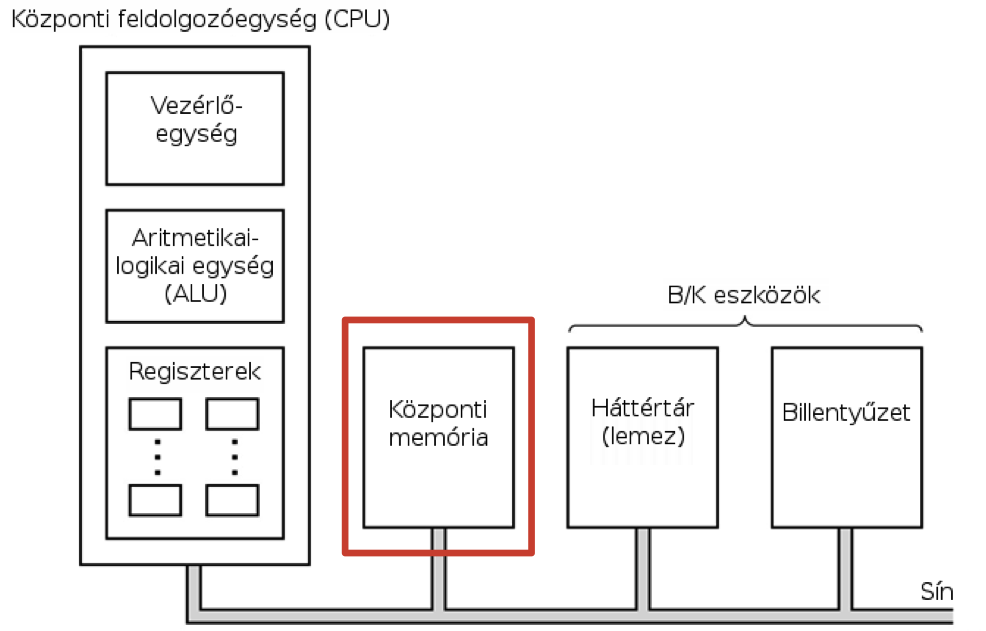
\includegraphics[width=\textwidth]{neumann}
\end{figure}

A \emph{központi memória} a program kódját és adatait tartalmazza számokként tárolva. A \emph{központi feldolgozóegység} a központi memóriában tárolt program utasításait olvassa be és hajtja végre. A \emph{külső sín} a számítógép részegységeit köti össze; adatokat, címeket és vezérlőjeleket továbbít. A \emph{belső sín} a CPU részei közötti kommunikációt teszi lehetővé. A \emph{bemeneti-kimeneti eszközök} segítségével valósul meg a kapcsolat a felhasználóval és az adattárolás (háttértárolón).

Ezen kívül egyéb, a \emph{működést segítő eszközök} tartoznak a számítógéphez, mint például a gépház és a tápegység.

\subsubsection{Központi memória}

\paragraph{Felépítése} A tárolás alapegysége a \emph{bit}, mely 0 vagy 1 értéket vehet fel. Ezt elektronikusan az áram jelenlétével vagy hiányával ábrázolják. Legkisebb címezhető egysége a \emph{rekesz (cella)}, mely egymást követő biteket tartalmaz. Egy rekesz leggyakrabban 8 bites (\emph{bájt}), de korábban ettől eltérő csoportosítással is lehetett találkozni.

A memóriarekeszek tartalmát címük alapján érhetjük el. Egyes gépeken a memóriát egydimenziós tömbnek tekinthetjük, melynek indexei a memóriacímek. Máshol a kis címhossz miatt szegmensekre osztják a memóriát, és a szegmens és egy ennek kezdőpontjához képesti eltolás megadásával címezhetünk meg egy rekeszt (\emph{szegmens:offszet címzés}). Ezeken kívül számos egyéb címzési mód létezik.

A számítógép egy regiszterébe beférő bájtokat \emph{szónak} nevezzük. A szó tehát 32-bites rendszeren 4, 64-bitesen 8 bájtot jelent. Sok gépi kódú utasítás teljes szavakkal dolgozik.A memóriában általában tetszőleges bájtot megcímezhetünk, de a szóhatáron kezdődő címek elérése gyorsabb. A fordítóprogramok általában képesek szóhatárra igazítani az adatokat.

A rekeszek adatokat (pl. egész, lebegőpontos, BCD szám, karakterkód, stb.) vagy gépi kódot tartalmazhatnak. A gépi kódú utasítások és ezek operandusai is számok.

\paragraph{Felosztása} A memória nagy részét a programok szabadon használhatják, bizonyos címterületek azonban a hardverrel való kapcsolattartásra vannak fenntartva. Bizonyos címek meghatározhatják egyes címterületek tartalmát (pl. RAM vagy ROM legyen ott elérhető).

\paragraph{Mérete} Korábban pár kilobájtos, megabájtos volt, ma több gigabájt az általános.

\subsection{Utasítás-végrehajtás. Utasítás- és processzorszintű párhuzamosság. RISC és CISC. Korszerű számítógépek tervezési elvei.}

\subsubsection{Processzorok}

A \emph{CPU} (Central Processing Unit, Központi Feldolgozóegység) feladata a központi memóriában tárolt programok végrehajtása. Ez az utasítások beolvasását, vizsgálatát, majd egyenkénti elvégzését jelenti.

A számítógép komponenseit \emph{sín} (bus) köti össze, ez cím-, adat- és vezérlőjeleket továbbító párhuzamos vezetékek kötege.

A CPU több önálló részegységből áll. A \emph{vezérlőegység} (Control Unit, CU) beolvassa az utasításokat a központi memóriából, és eldönti, hogy milyen típusúak. Az \emph{aritmetikai-logikai egység} (Arithmetic Logic Unit, ALU) az utasítások végrehajtásához szükséges matematikai és logikai műveleteket végzi el.

A CPU-ban kis méretű, nagy sebességű memóriarekeszek, regiszterek is vannak, midegyiknek meghatározott mérete és funkciója van. Általában minden regiszter azonos méretű. A legfontosabb regiszter a \emph{programszámláló} (Program Counter, PC), amely a következő végrehajtandó utasítás memóriacímét tartalmazza. Az \emph{utasításregiszterben} (Instruction Register, IR) pedig az épp végrehajtott utasítást találjuk.

\subsubsection{Utasítás-végrehajtás}

\begin{figure}[htbp]	
	\centering
		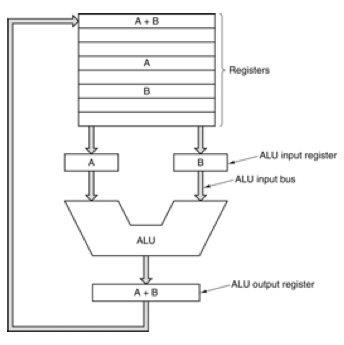
\includegraphics[width=10cm]{adatut}
	\caption{Adatút\label{fig:adatut}}	
\end{figure}

A~\ref{fig:adatut}. ábra az utasítás-végrehajtás úgynevezett \emph{adatciklusát} ábrázolja. Az utasítás (jelen esetben az összeadás) A és B operandusai az általános regiszterekből az ALU bemeneti regisztereibe kerülnek, majd az ALU elvégzi rajtuk a kívánt műveletet. Az eredmény a kimeneti regiszterbe íródik, ahonnan az egyik általános regiszterbe íródik vissza. Az adatok által a ciklusban megtett utat nevezzük \emph{adatútnak}.

A CPU \emph{betöltő-dekódoló-végrehajtó} ciklusának lépései a következők:

\begin{enumerate}
	\item Soron következő utasítás beolvasása a memóriából az utasításregiszterbe
	\item Az utasításszámláló beállítása a következő utasítás címére
	\item A beolvasott utasítás típusának meghatározása
	\item Ha az utasítás a memória egyik szavát használja, helyének megkeresése
	\item Ha szükséges, a memóriaszó beolvasása az egyik CPU-regiszterbe
	\item Az utasítás végrehajtása
	\item Vissza az 1. pontra
\end{enumerate}

A memória elérése lassú, az utasítás és az adatok beolvasása közben a CPU többi része kihasználatlanul marad. Ennek részleges kiküszöbölésére többféle gyorsítási lehetőség kínálkozik:

\begin{itemize}
	\item Órajel frekvenciájának növelése (korlátozott)
	\item Utasításszintű párhuzamosság
		\begin{itemize}
			\item Csővezeték
			\item Szuperskaláris architektúrák
		\end{itemize}
	\item Processzorszintű párhuzamosság
		\begin{itemize}
			\item Tömbszámítógépek
			\item Multiprocesszorok
			\item Multiszámítógépek
		\end{itemize}
\end{itemize}

Mielőtt továbbmennénk, definiálnunk kell két fogalmat. A \emph{késleltetés} egy utasítás végrehajtásának időigényét, a \emph{processzor sávszélessége} (processzor sávszélessége, MIPS, Million Instructions Per Second) pedig azt jelenti, hogy a processzor másodpercenként hánymillió utasítást képes végrehajtani.

\subsubsection{Utasításszintű párhuzamosság}

\begin{figure}[htbp]	
	\centering
		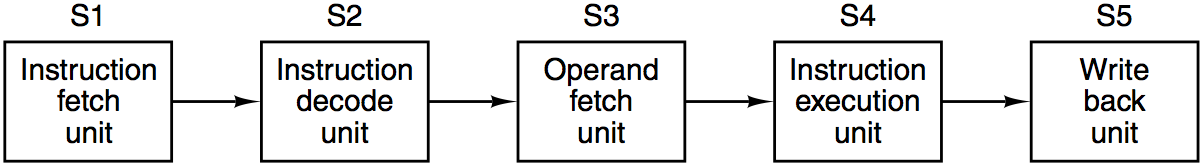
\includegraphics[width=\textwidth]{csovezetek}
	\caption{Példa csővezetékre\label{fig:csovezetek}}	
\end{figure}

\paragraph{Csővezetékek} A processzorokban már nagyon korán megjelent az \emph{előolvasási puffer} (prefetch buffer), egy olyan regisztercsoport, amibe a gép már az utasítás végrehajtásának vége előtt beolvassa a következő utasítást. Az előolvasás a végrehajtást így két részre osztja: a beolvasásra és magára a végrehajtásra.

A \emph{csővezeték} (pipeline) fogalma ezt a stratégiát fejleszti tovább; az utasítás-végrehajtást it sok (akár 12) részre is felosztják. Minden részlépést párhuzamos működésre képes, dedikált áramkörök hajtanak végre. A~\ref{fig:csovezetek}. ábrán egy ötfázisú csővezeték látható. A végrehajtás fázisai:

\begin{enumerate}
	\item Utasítás beolvasása a memóriából, majd pufferbe helyezése
	\item Utasítás típusának és operandusainak meghatározása
	\item Operandusok megkeresése és beolvasása a regiszterekből vagy a memóriából
	\item Az utasítás végrehajtása (tipikusan az operandusokat az adatúton végighajtva)
	\item Az eredmény beírása a megfelelő regiszterbe
\end{enumerate}

A~\ref{fig:csovezetek_vegrehajtas}. ábra az idő függvényében ábrázolja a csővezeték működését. A csővezetékezés módszere továbbfejleszthető \emph{párhuzamos csővezetékek} alkalmazásával. Ekkor egy közös utasítás-beolvasó egység több, saját ALU-val rendelkező csővezetéket szolgál ki. Ez az elrendezés akkor teszi lehetővé a párhuzamos végrehajtást, ha a csővezetékek nem használnak közös erőforrásokat, és nem függenek egymás eredményétől. Ezt vagy a fordítóprogramnak kell garantálnia, vagy extra hardver detektálja és oldja fel az ütközéseket. Általában 2-4 csővezetéket használnak. A Pentium hasonló megoldást alkalmaz, itt a fő csővezetékbe bármilyen, a másodlagosba csak egész műveleteket végző utasítás kerülhet.

\begin{figure}[htbp]	
	\centering
		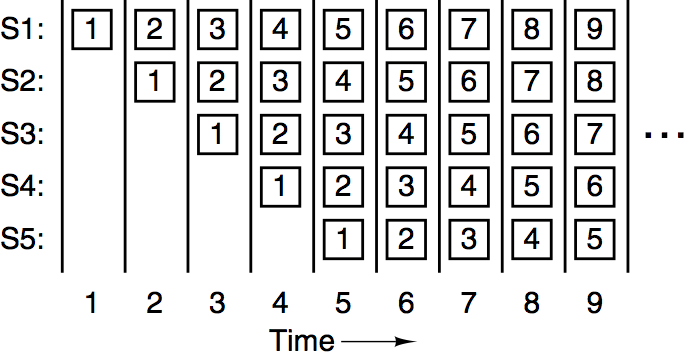
\includegraphics[width=10cm]{csovezetek_vegrehajtas}
	\caption{Csővezeték működése\label{fig:csovezetek_vegrehajtas}}	
\end{figure}

A csővezetékezés kompromisszum a késleltetés és a sávszélesség között. A sávszélesség nő, mert másodpercenként ötször annyi utasítás végrehajtása ér véget, mint egyébként. Viszont a késleltetés is nő, mert egy utasítást sokszor tovább tart végrehajtani.

\paragraph{Szuperskaláris architektúrák} Kettőnél több csővezeték hozzáadása már túl sok és túl bonyolult hardvert igényel, ezért ehelyett egy másik megoldást alkalmaznak. A processzorban csak egy csővezeték van, viszont ez több működési egységgel is rendelkezik, ahogy az a~\ref{fig:szuperskalaris}. ábrán látható. Az ilyen processzorok jellemzője, hogy egy órajelciklus alatt több utasítás végrehajtását is elkezdhetik. A kulcsgondolat tehát, hogy az utasításkiadás sebessége sokkal nagyobb lehet, mint a végrehajtásuké, mert ez utóbbit több részegység párhuzamosan végzi.

\begin{figure}[htbp]	
	\centering
		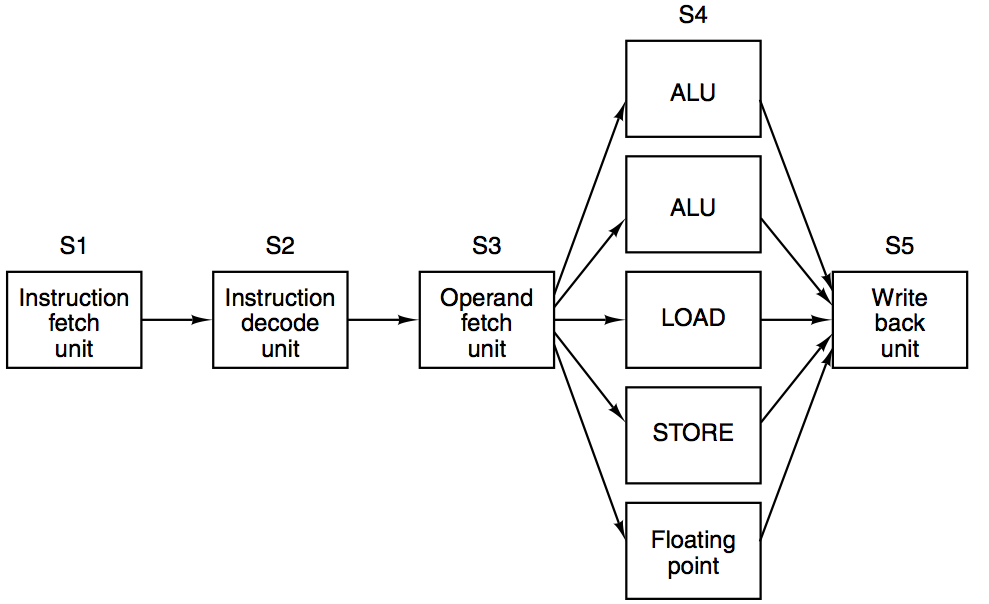
\includegraphics[width=\textwidth]{szuperskalaris}
	\caption{Szuperskaláris processzor öt működési egységgel\label{fig:szuperskalaris}}	
\end{figure}

\subsubsection{Processzorszintű párhuzamosság}

\paragraph{Tömbszámítógépek} Ha egy feladat megoldásához eltérő adatokon mindig ugyanazt a műveletet kell elvégezni, ezt a tulajdonságot kihasználhatjuk a megoldás párhuzamosítására. A \emph{tömbprocesszorokban} egyetlen vezérlőegység processzorok tömbjének egyszerre adja ki az utasításokat, melyeket azok a saját memóriájukból beolvasott, eltérő adatokon hajtanak végre. A \emph{vektorprocesszor} ettől abban tér el, hogy az összes összeadási műveletet egyetlen, erősen csővezetékezett összeadó végzi.

\paragraph{Multiprocesszorok} Közös memóriát használnak, ezért a processzorok együttműködése külön vezérlést igényel. A processzoroknak saját memóriája is lehet. Közösen használt sínrendszerük van, mely teljesítmény szempontjából gyakran szűk keresztmetszet. Jellemzően párszáz CPU-ból állnak. Könnyebb programozni, nehezebb megépíteni.

\paragraph{Multiszámítógépek} Nincs közös sínük, a processzorok közötti kommunikáció üzenetküldéssel valósul meg. Általában nincs minden gép összekötve egymással, például fastruktúrába, 2D, 3D rácsba vagy gyűrűbe szervezik őket. Ez azt eredményezi, hogy egy üzenetnek általában több számítógépen is át kell haladnia. Tízezer processzort is gond nélkül összekapcsoltak már ezzel a módszerrel. Nehezebb programozni, könnyebb megépíteni.

\subsubsection{CISC és RISC processzorok}

\paragraph{RISC (Reduced Instruction Set Computer)} Csökkentett utasításkészletű számítógép, csak az adatút egyszeri bejárásával végrehajtható utasításokat ismer. Tipikusan kb. 50 elemű utasításkészlet, jobb teljesítmény.

\paragraph{CISC (Complex Instruction Set Computer)} Összetett utasításkészletű számítógép, a gépi kódú utasításokat mikroprogram interpretálja. Ez az architektúra lassabb végrehajtást eredményez.

Az Intel processzorok eleinte CISC architektúrájúak voltak, később ebbe (a 80486-os típustól kezdve) a leggyakoribb utasítások végrehajtására integráltak egy RISC magot.

\subsubsection{Korszerű számítógépek tervezési elvei}

\begin{itemize}
	\item \emph{Minden utasítást közvetlenül a hardver hajtson végre.} A gyakran használtakat mindenképpen; az interpretált mikroutasításokat kerülni kell.
	\item \emph{Maximalizálni kell az utasítások kiadási ütemét.} Törekedni kell a párhuzamos utasításkiadásra.
	\item \emph{Az utasítások legyenek könnyen dekódolhatók.} Kevés mezőből álljanak, legyenek szabályosak, egyforma hosszúak.
	\item \emph{Csak a betöltő és a tároló utasítások hivatkozzanak a memóriára.} Törekedni kell a párhuzamos utasításkiadásra.
	\item \emph{Sok regiszter legyen.} A számítások során ne kelljen a lassú memóriába írni.
\end{itemize}

\section{Előadás}

\subsection{Számrendszerek, átváltások, egész számok ábrázolása, bináris aritmetika.}

\subsubsection{Számrendszerek}

A tízes számrendszerbeli számok számjegyei mindig a tíz valamely hatványának többszörösét jelentik. Általánosan így írhatunk fel egy tízes számrendszerbeli helyiértékes számot:

$$N = 10^{n} d_n + \dots + 10^3 d_3 + 10^2 d_2 + 10^1 d_1 + 10^0 d_0 + 10^{-1} d_{-1} + 10^{-2} d_{-2} + \dots + 10^{-k} d_{-k}$$

$$N = \sum_{i=-k}^{n} 10^i d_i\quad0 \leq d < 10$$

$N$ itt a szám értékét, $d_{-k} \dots d_n$ a számjegyeket jelenti. A helyiértékes számírás alapszáma a 10-től eltérő is lehet. Ha az alapszámot $b$-nek nevezzük, a számérték:

$$N = \sum_{i=-k}^{n} b^i d_i\quad0 \leq d < b$$

A tízesen kívül az informatikában fontos számrendszer a \emph{kettes (bináris)}, a \emph{nyolcas (oktális)} és a \emph{tizenhatos (hexadecimális)}. A kettes számrendszer számjegyei megfeleltethetők a biteknek, ezért a digitális számítógép binárisan számol. Egy oktális számjegy 3, egy hexadecimális 4 bináris számjegynek felel meg, ezért ezek között nagyon egyszerű az átalakítás. A 9-nél nagyobb hexadecimális számjegyeket növekvő sorrendben az A-F betűkkel jelöljük.

\subsubsection{Átváltások számrendszerek között}

Ha az egyik számrendszer alapszáma hatványa a másiknak, egyszerű az átváltás: az alacsonyabb alapszámú számjegyek csoportjai egymás után megfeleltethetők magasabb alapszámú számjegyeknek. A csoportosítás mindkét irányban a tizedesvesszőtől indul. Ugyanazt a bináris számot például így alakíthatjuk oktális és hexadecimális számmá:

$$0\underbrace{0 0 1}_1 \underbrace{1 0 0}_4 \underbrace{1 0 1}_5 \underbrace{0 0 1}_1 \underbrace{0 0 0}_0 , \underbrace{1 0 1}_5 \underbrace{1 0 1}_5 \underbrace{1 0 0_2}_4 = 14510,554_8$$

$$\underbrace{0 0 0 1}_1 \underbrace{1 0 0 1}_9 \underbrace{0 1 0 0}_4 \underbrace{1 0 0 0}_8 , \underbrace{1 0 1 1}_B \underbrace{0 1 1 0}_6 0_2 = 1948,B6_{16}$$

Oktális és hexadecimális számrendszerek között úgy válthatunk legegyszerűbben, hogy a számot először binárisan írjuk fel.

\begin{figure}[htbp]	
	\centering
		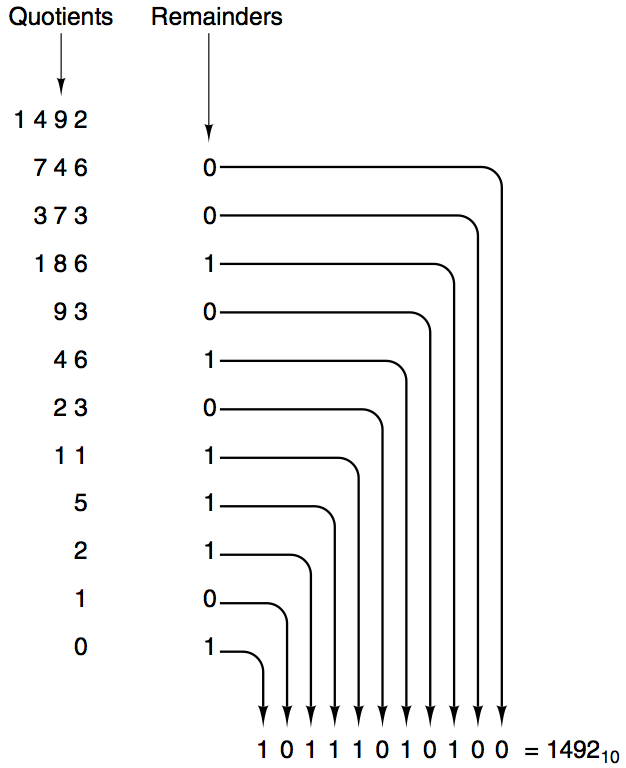
\includegraphics[width=8cm]{valtas_tizes_kettes}
	\caption{Váltás tízesből kettes számrendszerbe\label{fig:valtas_tizes_kettes}}	
\end{figure}

Egész értéket tízesből kettes számrendszerbe úgy váltunk, hogy a decimális értéket osztjuk 2-vel, majd feljegyezzük a hányados egészrészét és a maradékot. Ezt addig ismételjük, amíg a hányados 0 nem lesz. A bináris számjegyek az osztások maradékai lesznek, a legkisebb helyiértékre az első osztás maradéka kerül.

Decimális szám törtrészét úgy váltjuk binárisba, hogy a számot minden lépésben megszorozzuk kettővel. Ha a kapott szám 1, 1-es bináris számjegyet írunk, és az algoritmusnak vége. Ha 1-nél nagyobb, 1-es számjegyet írunk, kivonunk a számból 1-et, majd az 1. lépéssel folytatjuk. Ha 1-nél kisebb, akkor 0-s számjegyet írunk, majd folytatjuk az 1. lépéssel. Az első szorzás eredménye a legnagyobb helyiértékű számjegyet adja. Előfordul, hogy soha nem fejeződik be az algoritmus, végtelen kettedestörtet kapunk.

Kettesből tízes számrendszerbe úgy váltunk, hogy a legnagyobb helyiértékű bináris számjegytől indulva a számjegyhez hozzáadjuk az eddigi eredmény kétszeresét (ami először 0). Ezt a lépést addig ismételjük, amíg a számjegyek el nem fogynak, az utolsó végeredmény a tízes számrendszerbeli alak.

\begin{figure}[htbp]	
	\centering
		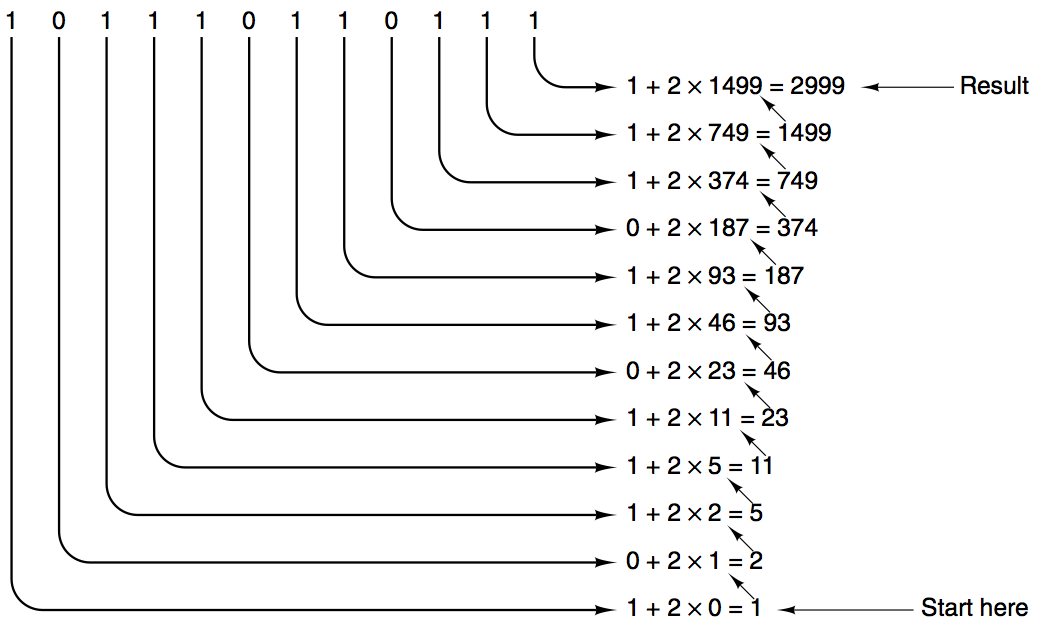
\includegraphics[width=12cm]{valtas_kettes_tizes}
	\caption{Váltás kettesből tízes számrendszerbe\label{fig:valtas_kettes_tizes}}	
\end{figure}

\subsubsection{Véges pontosságú számábrázolás}

A központi memória véges számú rekeszből áll, ezért a számítógépek általában rögzített számú bájton tárolják a számokat. Fix bitszélességen azonban csak adott értéktartomány ábrázolható, véges pontossággal.

A véges pontosságú számábrázolás új problémákhoz vezet: amikor a művelet eredménye nagyobb az ábrázolható tartományon, \emph{túlcsordulás}, amikor kisebb, \emph{alulcsordulás} következik be.

\subsubsection{Egész számok ábrázolása}

\paragraph{Nem negatív egészek} Bitek helyiértékének megfelelően ábrázoljuk őket kettes számrendszerbeli számként.

\paragraph{Binárisan kódolt decimális (BCD)} 4 (pakolt) vagy 8 (pakolatlan) bit jelöl egy decimális számjegyet. 4-bites reprezentáció esetén 100, 8-bitesnél 10 különböző szám ábrázolható így egy bájton. Bizonyos értékek nem hordoznak jelentést (pl. a 1011) -- a lehetséges értékeket pazaroljuk.

\paragraph{Negatív egész számok}

\subparagraph{Előjeles abszolútérték} Az előjelet a legfelső biten tároljuk (0 -- pozitív, 1 -- negatív). A további bitek a szám abszolútértékét tartalmazzák. Problémát okoz a 0 kétféle lehetséges ábrázolása ($+0$ és $-0$).

\subparagraph{Egyes komplemens} Az előjelet itt is a legfelső biten tároljuk. A további bitek a szám értékét tartalmazzák, de ha a szám negatív, bitenként negáljuk őket.

\subparagraph{Kettes komplemens} Úgy képezzük, hogy az egyes komplemens alakhoz $1$-et adunk. Ha a bal szélső bitnél átvitel jelenik meg, eldobjuk. A $0$ érték így csak egyféleképpen ábrázolható, viszont az ábrázolási tartomány nem szimmetrikus (bájtnál $-128$ és $+127$ között).

\subparagraph{$2^{m-1}$ többletes} Itt $m$ a bitek számát jelenti. $m=8$ esetén így 128 többletes ábrázolást alkalmazunk. A reprezentációt úgy kapjuk, hogy a többletes értékét hozzáadjuk az ábrázolandó számhoz. Így tehát a negatív számok képe kisebb, a nulláé egyenlő, a pozitívaké nagyobb a többletesnél. A kettes komplemenstől csak abban tér el, hogy az előjelbit fordított. Lebegőpontos számok kitevőjéhez használják.

\subsubsection{Bináris aritmetika}

A bináris számok összeadása ugyanúgy történik, mint a decimálisaknál. Az utolsó átvitelt az egyes komplemensnél hozzáadjuk a jobb szélső bithez, a kettesnél eldobjuk. Általános szabály, hogy ha a két tag ellentétes előjelű, nem lesz túlcsordulás, viszont ha előjelük megegyezik, az eredményé viszont ellentétes, akkor biztos, hogy túlcsordulás következett be.

\subsection{Lebegőpontos számok ábrázolása.}

\subsubsection{Törtszámok reprezentációja}

A törtszámok általános alakban az $n=f \cdot 10^e$ alakban írhatók fel, ahol $f$ a \emph{törtrész} vagy \emph{mantissza}, $e$ pedig a \emph{kitevő} vagy \emph{exponens}. Számítógépeken a tízes helyett 2-, 4-, 8- vagy 16-os alapot használnak.

A \emph{normalizált} vagy \emph{normálalak} azt az alakot jelenti, ahol az első nem nulla számjegy áll az egyesek helyén. A normálalakot a 10-estől eltérő számrendszerekben is értelmezzük.

Két fogalmat definiálunk a törtszámok reprezentációinak jellemzésére.
\begin{description}
	\item[Nagyságrend:] A kitevő jegyeinek száma határozza meg. Minél nagyobb, annál nagyobb az ábrázolható maximális érték.
	\item[Pontosság:] A törtrész jegyeinek száma határozza meg. Minél nagyobb, annál finomabb az ábrázolás ``felbontása'', vagyis annál kisebb a különbség két egymás melletti ábrázolt szám között.
\end{description}
Ebből láthatjuk, hogy az egészekhez hasonlóan a lebegőpontos ábrázolásnál is az $\mathbb{R}$ valós számhalmaznak csak egy részhalmazát tudjuk ábrázolni (hiszen két valós szám között végtelen sok újabbat találunk). Azt is fontos megjegyezni, hogy az ábrázolási pontosság eltérő nagyságrendű értékeknél más és más, nem egyenletes.

\subsubsection{Az IEEE 754-es lebegőpontos szabvány (1985)}

Kettes hatványalapot használ. Háromféle pontosságú ábrázolást definiál:
\begin{description}
	\item[Egyszeres pontosság:] 32 bit -- 1 előjelbit, 8-bites kitevő, 23-bites törtrész. Decimális kiterjedés: kb. $10^-38$-tól $10^38$-ig.
	\item[Dupla pontosság:] 32 bit -- 1 előjelbit, 11-bites kitevő, 52-bites törtrész. Decimális kiterjedés: kb. $10^-308$-tól $10^308$-ig.
	\item[Kiterjesztett pontosság:] 32 bit -- kerekítési hibák csökkentésére használják a lebegőpontos aritmetikai egység belsejében.
\end{description}

A szabvány többféle numerikus típust definiál, ezek:

\vspace{3mm}
\begin{tabular}{c c c c}
	& \emph{előjel} & \emph{kitevő} & \emph{törtrész}\\
	\textbf{Normalizált} & $\pm$ & $0<e<max$ & bitminta\\
	\textbf{Nem normalizált} & $\pm$ & 0 & nem 0 bitminta\\
	\textbf{Nulla} & $\pm$ & 0 & 0\\
	\textbf{Végtelen} & $\pm$ & $111\dots1$ & 0\\
	\textbf{Nem szám} & $\pm$ & $111\dots1$ & nem 0 bitminta\\
\end{tabular}
\vspace{3mm}

A \emph{normalizált} számok első számjegye 1 (a tizedesvesszőtől balra), ezért azt nem ábrázoljuk. Ezt \emph{szignifikánsnak} nevezzük (törtrész helyett). Az ábrázolt szám értéke:

$$\pm (1 + szign) \cdot 2^{e}$$

A \emph{nem normalizált} számok első számjegye 0, ezért azt nem ábrázoljuk. Az ábrázolt szám értéke itt:
$$\pm (0 + f) \cdot 2^{-126}$$
Ahol $f$ a törtrész, a kitevő pedig rögzítetten $-126$. Segítségével kezelhető az alulcsordulás: a normalizáltnál kisebb értékeket ábrázolhatunk.

A \emph{végtelen} és az \emph{érvénytelen} (nem szám) értékekkel végzett aritmetikának speciális szabályai vannak:
\begin{itemize}
	\item $n/0=\infty$, ahol $n$ egy szám
	\item $n/\infty=0$, ahol $n$ egy szám
	\item $\infty + N=\infty$, ahol $N$ bármi lehet
	\item $0/0=NaN$
\end{itemize}

\subsection{Szöveg kódolása. Bájtsorrend. Hibadetektáló és -javító kódok.}

\subsubsection{Szöveg kódolása}

\paragraph{ASCII (1963)} A bájtok értékei karaktereket jelentenek. A karakter lehet szám, a latin ábécé betűje, írásjel vagy vezérlőkód. Csak az alsó 7 bit használatos.

\paragraph{Kiterjesztett ASCII} A 128-255 közötti értékek is definiáltak, pl. nemzetközi karaktereket, szimbólumokat tartalmaznak. Még így is nagyon kevés a hely, ezért különféle kiterjesztett karakterkészleteket, ``kódlapokat'' használnak -- ez az \emph{ISO 8859}-es kódolási szabvány. Ez sem jelent tökéletes megoldást, egyszerre több nyelv karakterei, vagy a kínai, japán karakterek nem férnek bele.

\paragraph{Unicode (UTF) és ISO/EIC 10646 szabvány (1989-1990)} Az \emph{UTF-16} kódolás rögzítetten 16-bites (2-bájtos). \texttt{0} és \texttt{10FFFF} közötti kódok lehetségesek. A bájtsorrend architektúrafüggő, az opcionális BOM (Byte Order Mark) segítségével automatikusan megállapítható. Értéke \texttt{U+FEFF}. Az \emph{UTF-32} 4 bájton tárol egy karaktert, így a legnagyobb tárolható érték \texttt{7FFFFFFF}-re nő. A bájtsorrend itt is problémát jelent. Szövegek helyett inkább csak 1-1 karakter leírására használják.

\subsubsection{Bájtsorrend}

\begin{description}
	\item[Little-endian:] A szó \emph{alacsonyabb} helyiértékeinek bájtjai szerepelnek az alacsonyabb memóriacímeken.
	\item[Big-endian:] A szó \emph{magasabb} helyiértékeinek bájtjai szerepelnek az alacsonyabb memóriacímeken.
\end{description}

Eltérő bájtsorrendű rendszerek közöt a bitfolyamként továbbított adatok összekeverednek. \emph{Sorrendi} továbbításnál a bájttömbként tárolt stringek helyesen, a több bájton tárolt egész értékek helytelenül tárolódnak. \emph{A bájtokat megcserélve} a stringek karaktereinek (beleértve a \texttt{\textbackslash0} stringvégződést is!) sorrendje összekeveredik, de az egészek helyesen tárolódnak. Az alábbi megoldási lehetőségek vannak:
\begin{description}
	\item[Szöveges kódolás:] XML, JSON, stb. alkalmazása.
	\item[Bájtsorrend-jelölő érték használata:] Az adat elején egy olyan érték elhelyezése, amelyből megállapítható a bitfolyam bájtsorrendje (pl. Unicode esetén a \emph{Byte Order Mark} -- BOM, értéke \texttt{U+FEFF}).
\end{description}

\subsubsection{Hibadetektáló és -javító kódok}

A memória hibázhat, például hirtelen áramlökés vagy hardverhiba hatására. Ez, ha adatterületen történik, számítási hibához, ha kódterületen, hibás működéshez, lefagyáshoz vezethet. A hibák redundancia bevezetésével védhetők ki. \emph{Detekció} esetén a rendszer bizonyos hibákat képes észlelni és az aktuális program futását leállítani. \emph{Hibajavításnál} bizonyos hibák esetén helyreállítható a legvalószínűbb helyes bájtérték.

Egyszerű példa hibadetekcióra a \emph{paritásbit alkalmazása}. Tegyünk hozzá minden bájthoz egy kilencedik bitet, amely akkor legyen 1, ha a bájtban páratlan számú 1-es számjegy van (biztosítja, hogy a 9 biten mindig páros számú 1-es érték legyen). Ha a paritásbit értéke nem megfelelő, az memóriahibára utal. Módszerünk azonban korlátozott: csak páratlan számú bithibát tud detektálni, javításra pedig nem képes.

\begin{description}
	\item[Kódszó:] $m$ adatbit és $r$ ellenőrző bit $n=m+r$ bites együttese.
	\item[Hamming-távolság:] két bináris szám eltérő számjegyeinek száma.
	\item[Kód Hamming-távolsága:] Ha ismerjük az ellenőrzőbitek kiszámításának algoritmusát, megalkothatjuk az érvényes kódszavak teljes listáját. Keressük meg azt a két kódszót a listán, melyek Hamming-távolsága minimális; ez a teljes kód Hamming-távolsága.
\end{description}

Egy kód hibadetektáló és hibajavító tulajdonságai Hamming-távolságától függnek. Legalább $d$ darab bithiba detektálásához legalább $d+1$ távolságú kódolás szükséges, mert így $d$ bithiba egyetlen érvényes kódszót sem alakíthat át egy másikba. $d$ bithiba \emph{javításához} $2d+1$ távolságú kódolásra van szükség, mert így az érvényes kódok olyan távol vannak egymástól, hogy még $d$ darab változtatás után is közelebb van az eredeti kódszó, mint bármely másik.

Tegyük fel, hogy egy egybites hibákat kijavítani képes kódolást szeretnénk tervezni $m$ adatbit és $r$ ellenőrző bit használatával. A $2^m$ legális memóriaszó mindegyikétől pontosan $n$ darab illegális kódszó van 1 bit távolságra -- ezeket úgy kapjuk, hogy az $n$-bites kódszó bitjeit egyesével, sorban negáljuk. Így mind a $2^m$ legális szóhoz $n+1$ bitmintát kell rendelnünk ($n$ lehetséges hiba és a helyes minta). Mivel a bitminták teljes száma $2^n$, ezért a következőnek kell teljesülnie:
\begin{align*}
	(n + 1)2^m     & \leq 2^n     & (n = m + r)         \\
	(m + r + 1)2^m & \leq 2^{m+r} & (n^{a+b} = n^a n^b) \\
	(m + r + 1)2^m & \leq 2^m 2^r & : 2^m               \\
	m + r + 1      & \leq 2^r
\end{align*}
Ez az összefüggés alsó korlátot ad az egybites hibák javításához szükséges ellenőrzőbitek számára.

Az alsó korlátot \emph{Richard Hamming} algoritmusával (1950) el is lehet érni. Előbb azonban a négybites szavak hibajavító kódolását egy egyszerű grafikus példával illusztráljuk (ld.~\ref{fig:hibajavitas}. ábra). Az $A$, $B$ és $C$ halmazok metszeteibe a szó értékét ($1100$) írjuk, a metszeteken kívüli részekre pedig paritásbiteket helyezünk úgy, hogy minden halmazban páros számú $1$-es bit legyen. Ha az $AC$ területen hiba keletkezik, és a $0$-s bit $1$-esre változik, az $A$ és a $C$ halmazok paritása rossz lesz. Az egyetlen olyan egybites változtatás, amely helyreállítja a paritást, az $AC$ $0$-ra állítása. Így a számítógép az egybites memóriahibákat automatikusan helyre tudja állítani.

\begin{figure}[htbp]	
	\centering
		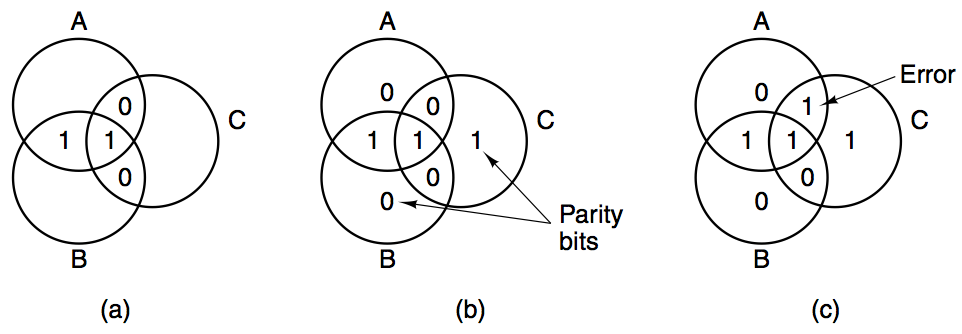
\includegraphics[width=\textwidth]{hibajavitas}
	\caption{(a) Az $1100$ kódolása. (b) Paritásbitek hozzáadva. (c) Hiba az AC-ben\label{fig:hibajavitas}}	
\end{figure}

A Hamming-algoritmussal bármekkora, $m$ hosszúsűgú memóriaszóhoz tudunk hibajavító kódot gyártani $r$ paritásbit hozzáadásával. A biteket 1-től (és nem 0-tól) számozzuk; az 1. bit a bal szélső (legnagyobb helyiértékű). Minden olyan bit, amelynek sorszáma a 2 hatványa, paritásbit, a több adatot tárol. Egy 16-bites szóhoz így például 5 paritásbitet adunk -- az 1, 2, 4, 8, 16 sorszámú bitek a paritásbitek. Így összesen 21-bites memóriaszót kapunk, 16 adat- és 5 paritásbittel. A példában páros paritást fogunk használni. A paritásbitek a következő biteket ellenőrzik:
\begin{align*}
	1 &\rightarrow 1, 3, 5, 7, 9, 11, 13, 15, 17, 19, 21 \\
	2 &\rightarrow 2, 3, 6, 7, 10, 11, 14, 15, 18, 19    \\
	4 &\rightarrow 4, 5, 6 7, 12, 13, 14, 15, 20, 21     \\
	8 &\rightarrow 8, 9, 10, 11, 12, 13, 14, 15          \\
	16 &\rightarrow 16, 17, 18, 19, 20, 21               \\
\end{align*}
Általánosan, a $b$-edik bitet azon $b_1, b_2, \dots, b_j$ bitek ellenőrzik, melyekre $b_1 + b_2 + \dots + b_j = b$. Például az 5. bitet az 1-es és a 4-es bitek ellenőrzik, mert $1+4=5$. A hibajavítás úgy történik, hogy kiszámoljuk a paritásokat, és összeadjuk a helytelen értékű paritásbitek sorszámát, így megkapjuk a negálandó bit sorszámát.

\begin{figure}[htbp]	
	\centering
		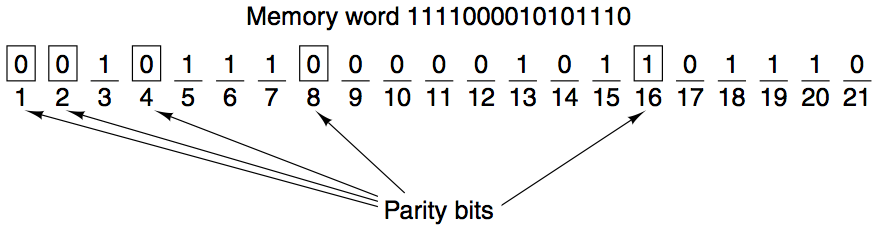
\includegraphics[width=\textwidth]{hamming}
	\caption{Hamming-kód az 1111000010101110 16-bites memóriaszóhoz 5 ellenőrző bit hozzáadásával.\label{fig:hamming}}	
\end{figure}

\section{Előadás}

\subsection{Kapuk és Boole-algebra. Tranzisztor, inverter, \textsc{nem-és} (\textsc{nand}) kapu, \textsc{nem-vagy} (\textsc{nor}) kapu, \textsc{és} (\textsc{and}), \textsc{vagy} (\textsc{or}) kapuk.}

\subsubsection{Kapuk és Boole-algebra}

A digitális árakörök $0$ és $1$ értékeit (valójában 0-1 és 2-5 volt közötti feszültséget jelentenek) megfeleltethetjük a \emph{Boole-algebra} logikai \textsc{hamis} és \textsc{igaz} értékeinek. Áramköri elemekből logikai kapukat (pl. \textsc{and}, \textsc{or}) építhetünk, melyekkel tetszőleges logikai függvény megvalósítható.

\subsubsection{Tranzisztor, inverter, logikai kapuk}

A tranzisztor árammal vezérelt kapcsolóként is használható. Állapota \emph{zárt}, ha $V_{be}$ bizonyos szint alatt van, ellenállása ilyenkor kvázi végtelen ($V_{ki} \approx V_{CC}$). Ha $V_{be}$ meghaladja a kritikus értéket, \emph{kinyit}, ekkor $V_{ki} = 0V$ lesz. Ha a logikai jel a $V_{be}$, egyetlen tranzisztor inverterként (\textsc{not}-kapu) működik. Két tranzisztor soros, illetve párhuzamos kapcsolásával \textsc{nand}- és \textsc{nor}-kaput építhetünk (ld.~\ref{fig:kapuk_tranzisztor}. ábra). Az összes kapu áramköri szimbóluma és igazságtáblája a~\ref{fig:kapuk}. ábrán látható.

\begin{figure}[htbp]
	\centering
		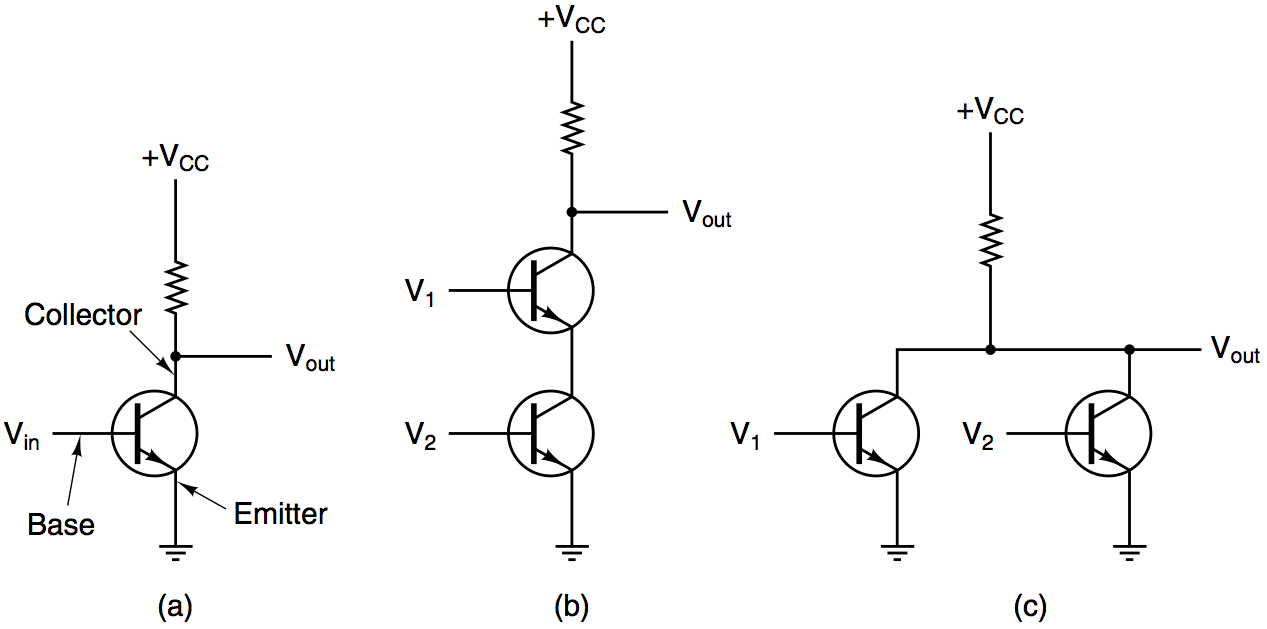
\includegraphics[width=\textwidth]{kapuk_tranzisztor}
	\caption{\textsc{not}-, \textsc{nand}- és \textsc{nor}-kapuk\label{fig:kapuk_tranzisztor}}
\end{figure}

\begin{figure}[htbp]
	\centering
		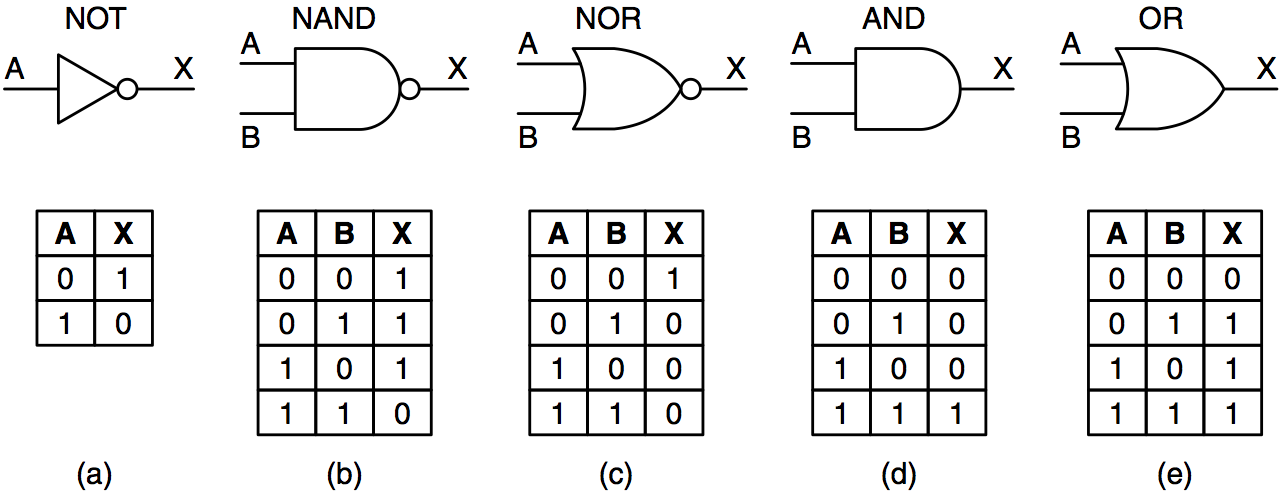
\includegraphics[width=\textwidth]{kapuk}
	\caption{Logikai kapuk áramköri szimbóluma és igazságtáblája.\label{fig:kapuk}}
\end{figure}

\subsection{Boole-algebra. Boole-függvények megvalósítása. Áramköri ekvivalencia.}

\subsubsection{Boole-algebra}

Kapuk kombinációjából felépíthető áramkörök leírására szolgál. A változók értéke és a függvények értékkészlete a ${0, 1}$ halmaz. A \emph{Boole-függvények} egy vagy több bemeneti változóból egy kimeneti értéket állítanak elő. A fügvényt \emph{logikai formulával} vagy \emph{igazságtáblával} definiáljatjuk. Utóbbi esetben $n$ bemenő változó esetén $2^n$ lehetséges kombinációra kell megadni a kimenő értékeket. A táblázat egy sora adott bemeneti értékek esetén megadja a függvényértéket.

Tekintsük példáula \emph{háromváltozós többségi logikai függvényt}. Ez ún. \emph{diszjunktív normálformával} megadva így néz ki:

$$M = f(A, B, C) = \bar{A}BC + A\bar{B}C + AB\bar{C} + ABC$$

A diszjunktív normálforma többváltozós függvényeknél sokkal kényelmesebb megadási mód, mint az igazságtábla.

\subsubsection{Boole-függvények megvalósítása}

Egy $n$-változós függvány legfeljebb $2^n$ darab $n$-változós logikai szorzat összege. Áramköri megvalósítása szabványos logikai kapuk segítségével történik, de fontos, hogy az absztrakt Boole-függvény és az elektronikus megvalósítás között különbség van. Utóbbi esetben a változókat elektromos jelek, a műveleteket pedig kapuk reprezentálják.

\begin{figure}[htbp]
	\centering
		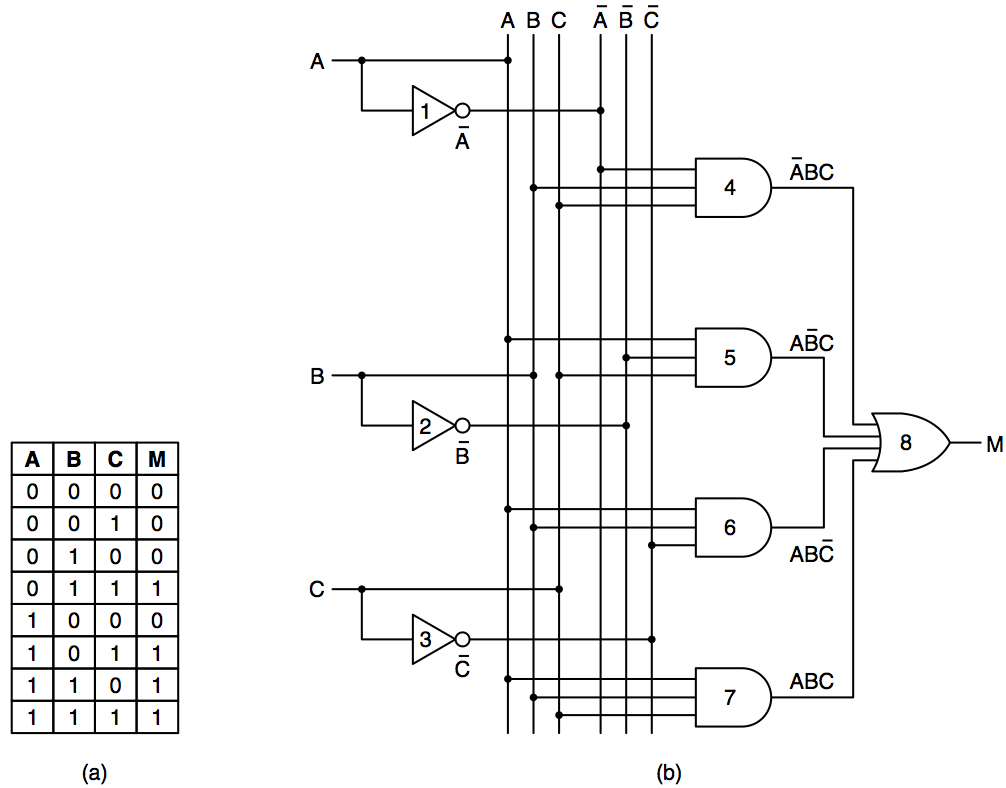
\includegraphics[width=\textwidth]{tobbsegifv}
	\caption{Többségi függvény (a) igazságtáblája és (b) áramköri megvalósítása.\label{fig:tobbsegifv}}
\end{figure}

\paragraph{Logikai függvény megvalósításának lépései}
\begin{enumerate}
	\item Felírjuk a függvény igazságtábláját
	\item \textsc{nem}-kapukkal előállítjuk minden bemenet negáltját
	\item Minden olyan sorhoz, amelynek eredményoszlopa $1$-est tartalmaz, \textsc{és}-kapukat helyezünk el
	\item Az \textsc{és}-kapukat összekötjük a megfelelő bemenetekkel
	\item Az összes \textsc{és}-kapu kimenetét bekötjük egy \textsc{vagy}-kapuba
\end{enumerate}

Az áramköröket kényelmesebb és hatékonyabb úgy megvalósítani, hogy csak egyféle kaput használunk. Ehhez ún. \emph{teljes} kapukkal kell dolgoznunk, melyekkel bármilyen Boole-függvény kiszámítható. Erre egyedül a \textsc{nem-és} és a \textsc{nem-vagy} kapuk képesek.

\begin{figure}[htbp]
	\centering
		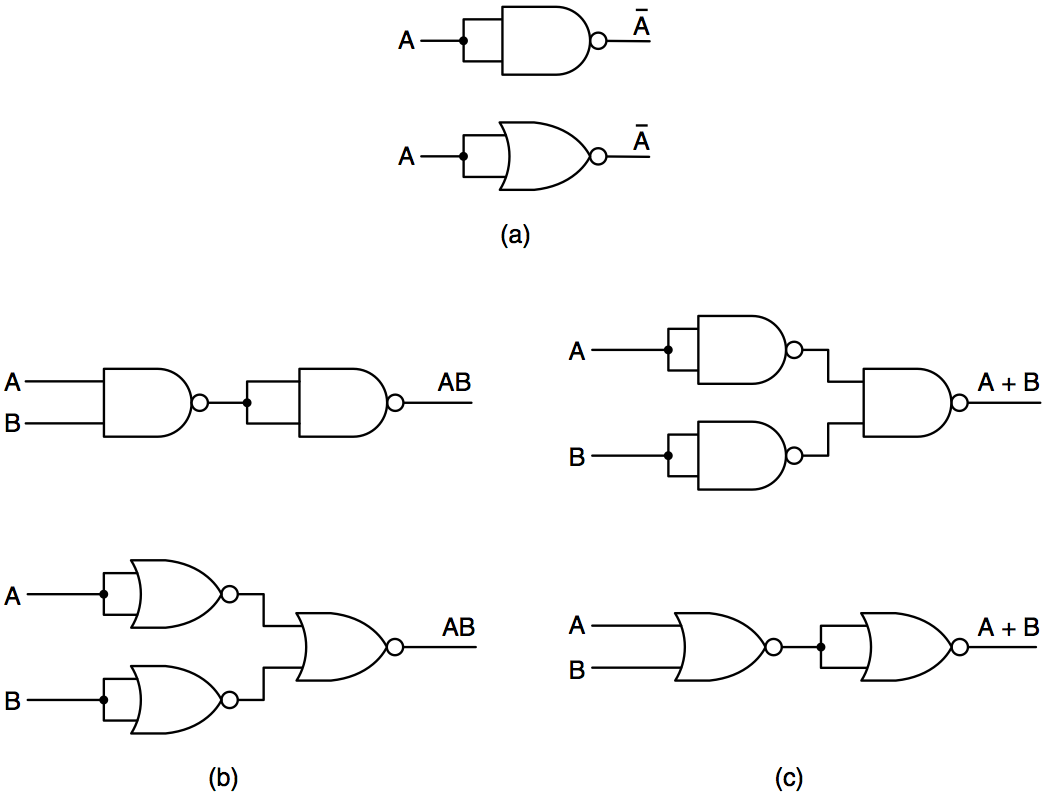
\includegraphics[width=\textwidth]{helyettesitokapuk}
	\caption{(a) \textsc{not}-, (b) \textsc{and}- és (c) \textsc{or}-kapuk megvalósítása \textsc{nand}- és \textsc{nor}-kapuk segítségével.\label{fig:helyettesitokapuk}}
\end{figure}

\subsubsection{Áramköri ekvivalencia}

Logikai függvények megvalósításakor mindig törekedni kell a kapuk számának csökkentésére. Így az alkatrész ára, a nyomtatott áramköri lap nagysága és az áramfogyasztás is csökken. Találni kell egy olyan függvényt, amely ugyanazt a függvényt számolja ki, mint az eredeti, de kevesebb kapuból áll -- ennek fontos eszköze a Boole-algebra. Az alábbi táblázat ennek legfontosabb szabályait mutatja be.

\vspace{3mm}
\begin{tabular}{l c c}
	\textbf{Név}          & \textbf{\textsc{és}-forma} & \textbf{\textsc{vagy}-forma} \\
	Identitásszabály      & $1A = A$                        & $0 + A = A$             \\
	Nullszabály           & $0A = 0$                        & $1 + A = 1$             \\
	Idempotens szabály    & $AA = A$                        & $A + A = A$             \\
	Inverzszabály         & $A\bar{A} = 1$                  & $A + \bar{A} = 1$       \\
	Kommutatív szabály    & $AB = BA$                       & $A + B = B + A$         \\
	Asszociatív szabály   & $(AB)C = A(BC)$                 & $(A+B)+C = A+(B+C)$     \\
	Disztribúciós szabály & $A + BC = (A + B)(A + C)$       & $A(B+C) = AB + AC$      \\
	Abszorpciós szabály   & $A(A + B) = A$                  & $A + AB = A$            \\
	De Morgan-szabály     & $\overline{AB}=\bar{A}+\bar{B}$ & $\overline{A+B}=\bar{A}\bar{B}$
\end{tabular}
\vspace{3mm}

\begin{figure}[htbp]
	\centering
		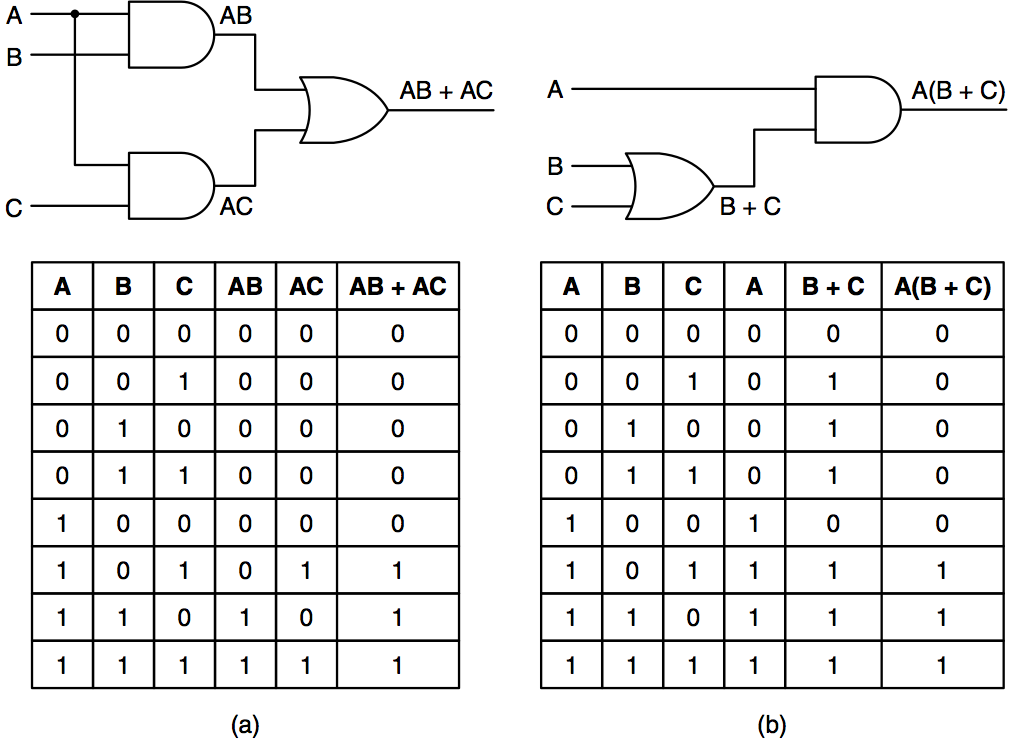
\includegraphics[width=10cm]{ekvivalencia}
	\caption{Példa ekvivalens áramkörökre.\label{fig:ekvivalencia}}
\end{figure}

Figyeljük meg, hogy minden szabálynak két formája van, és ezek egymásnak \emph{duálisai} -- az \textsc{és} és \textsc{vagy} műveletek, illetve a $0$ és $1$ igazságértékek cseréjével egymásból előállíthatók. A szabálok igazságtáblájukkal bizonyíthatók. A fenti szabályokon kívül fontos még a De Morgan-szabály kiterjesztése:
$$\overline{ABC} = \bar{A} + \bar{A} + \bar{C}$$

A szabályok alapján alternatív áramköri szimbólumokat adhatunk meg néhány ismert kapuhoz (ld.~\ref{fig:alternativszimbolumok}. ábra). Az, hogy az egyes feszültségértékekhez milyen igazságértéket rendelünk, tulajdonképpen önkényes, ahogy azt a~\ref{fig:pozneglogika}. ábra is mutatja. Újabb példa az áramköri ekvivalenciára az \textsc{xor}-művelet \textsc{nand}-kapukkal történő megvalósítása (ld.~\ref{fig:xoralternativak}. ábra).

\begin{figure}[htbp]
	\centering
		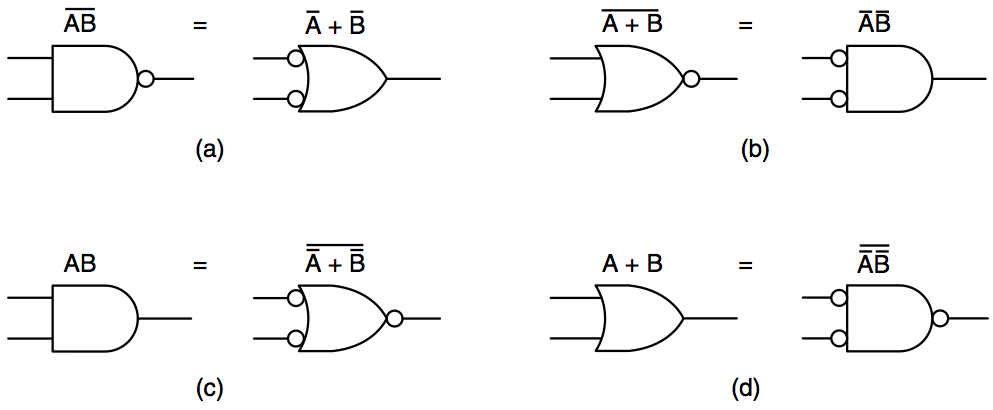
\includegraphics[width=12cm]{alternativszimbolumok}
	\caption{Új áramköri szimbólumok.\label{fig:alternativszimbolumok}}
\end{figure}

\begin{figure}[htbp]
	\centering
		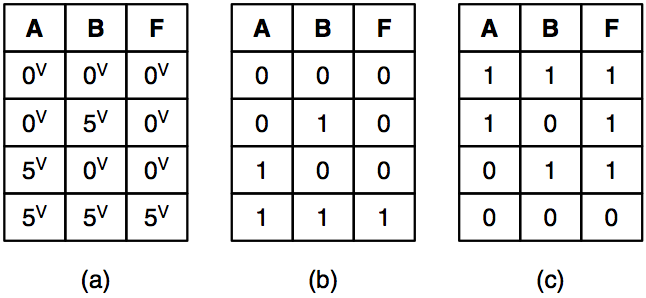
\includegraphics[width=8cm]{pozneglogika}
	\caption{(a) Elektronikus karakterisztika, (b) pozitív és (c) negatív logika.\label{fig:pozneglogika}}
\end{figure}

\begin{figure}[htbp]
	\centering
		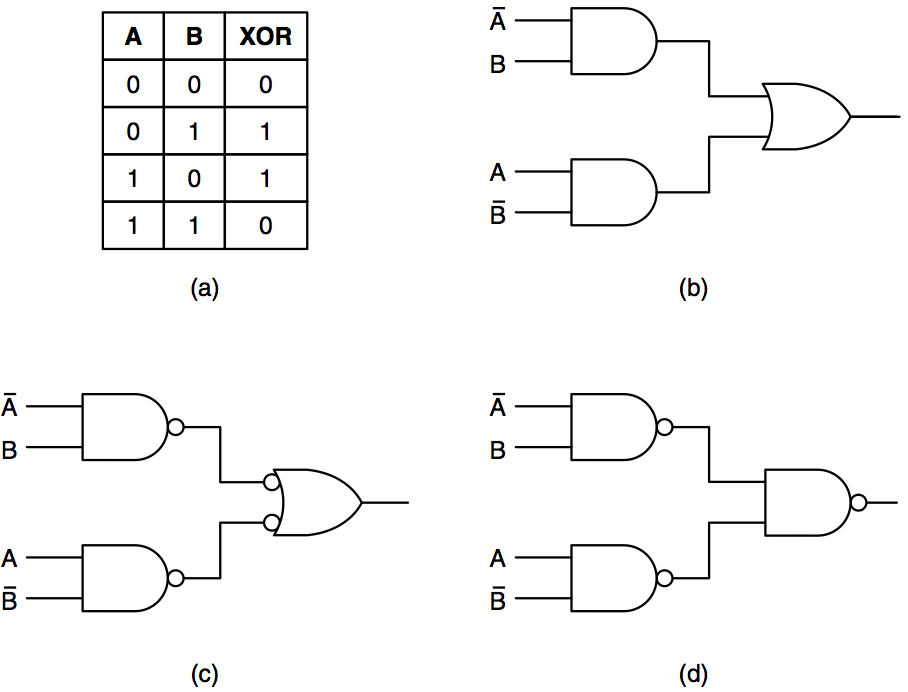
\includegraphics[width=10cm]{xoralternativak}
	\caption{\textsc{xor}-művelet igazságtáblája és háromféle áramköri megvalósítása.\label{fig:xoralternativak}}
\end{figure}

\subsection{Alapvető digitális logikai áramkörök. Integrált áramkörök. Kombinációs áramkörök.
Multiplexerek, demultiplexer. Dekódolók. Összehasonlítók.}

\subsubsection{Alapvető digitális logikai áramkörök}

Manapság kevés áramkört építenek különálló kapukból, inkább számos kaput tartalmazó építőblokkokat alkalmaznak. Ilyenek az \emph{integrált áramkörök} (Integrated Circuit, IC). Tokjuk téglatest alakú, műanyagból vagy kerámiából készül. Lábaikkal kapcsolódnak az áramkör többi eleméhez, melyeket vagy beforrasztanak az áramköri lapba, vagy foglalatba helyeznek. Minden lábuk egy kapu bemenete vagy kimenete. A kétsoros lábazást és a belső integrált áramkört együtt \emph{Dual Inline Package}-nek (DIP) nevezik.

\subsubsection{Integrált áramkörök}

\begin{description}
	\item[SSI (Small Scale Integration):] kis integráltásgú áramkör, 1-10 kaput tartalmaz.
	\item[MSI (Medium Scale Integration):] közepes integráltságú, 10-100 kapu.
	\item[LSI (Large Scale Integration):] nagy integráltságú, 100-100\,000 kapu.
	\item[VLSI (Very Large Scale Integration):] nagyon nagy integráltásg, több mint 100\,000 kapu.
\end{description}

A~\ref{fig:ssi}. ábra egy 4 \textsc{nand}-kaput tartalmazó SSI-lapkát ábrázol. A kapukhoz 12 láb tartozik, kapunként két bemenet és egy kimenet. Ezen kívül a $V_{CC}$ feszültség és a föld (GND) kap egy-egy lábat.

\begin{figure}[htbp]
	\centering
		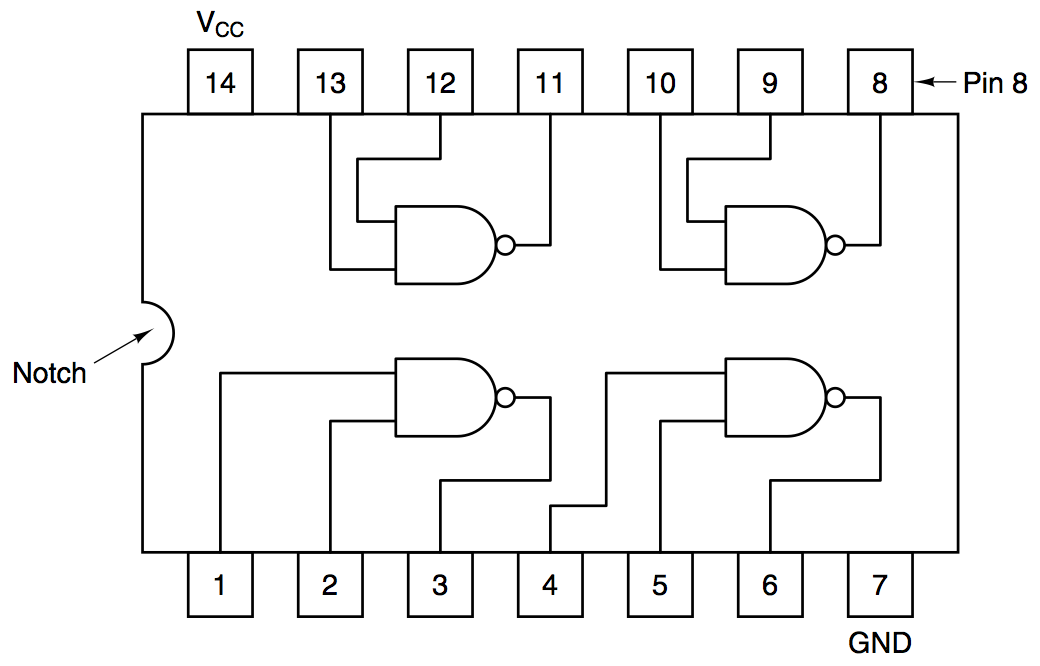
\includegraphics[width=6cm]{ssi}
	\caption{4 \textsc{nand}-kaput tartalmazó SSI-lapka.\label{fig:ssi}}
\end{figure}

Az \emph{ideális kapu} kimenete azonnal előáll, amint a bemenetet alkalmazzuk, viszont a valóságban a lapkáknak véges kapukésleltetésük van. Ez tartalmazza a jel terjedési és a kapu kapcsolási idejét is.

A mai VLSI-lapkákon kb. 10 millió tranzisztor van, ez kb. 5 millió kapunak felel meg. Ezek független használatához 15\,000\,002 lábra lenne szükség, ami nyilvánvalóan kivitelezhetetlen. Így ezek nagy kapu/láb arányú áramkörök, csak korlátozott számú kapcsolatuk lehetséges a külső áramkörrel.

\subsubsection{Kombinációs áramkörök}

Ezek több bemenettel és kimenettel rendelkező logikai áramkörök, amelyek kimenetét egyértelműen meghatározzák a bemenetek (nem minden áramkör ilyen, pl. a memóriaelemeknél az állapot is számít).

\subsubsection{Multiplexerek, demultiplexer}

\paragraph{Multiplexer} Olyan áramkör, amelynek $n$ vezérlőbemenete, $2^n$ adatbemenete és $1$ adatkimenete van. A vezérlőbemenetek egy adatbemenetet címeznek meg, ennek jele jut az adatkimenetre (ld.~\ref{fig:multiplexer}. ábra). $n=3$ esetén áram és föld lábakkal együtt egy 14 lábas tokban helyezhető el. Bármely $n$-változós igazságtábla megvalósítható vele, például a többségi függvény (ld.~\ref{fig:tobbsegifvmux}. ábra).

\begin{figure}[htbp]
	\centering
		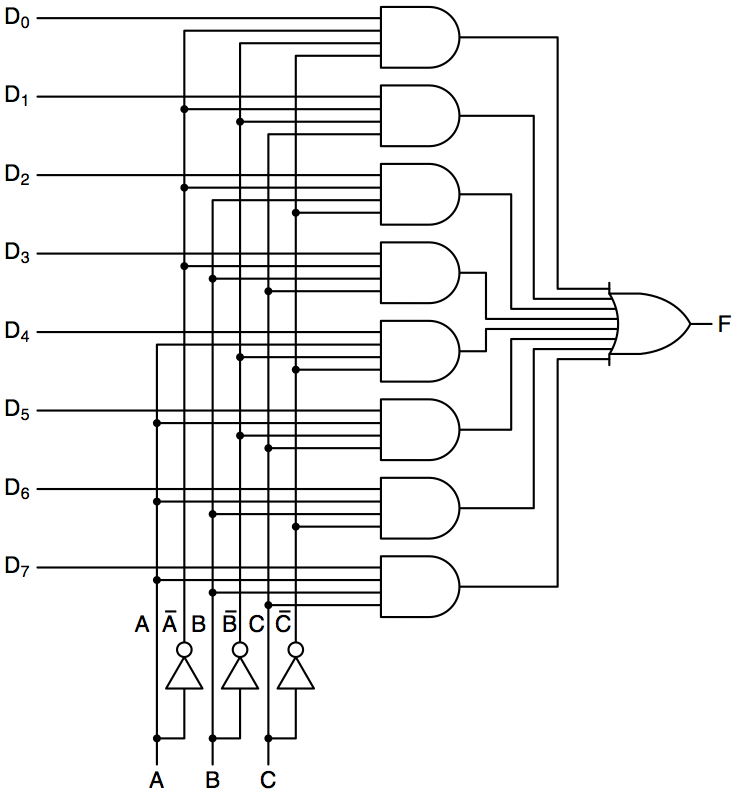
\includegraphics[width=10cm]{multiplexer}
	\caption{Multiplexer logikai áramköre.\label{fig:multiplexer}}
\end{figure}

\begin{figure}[htbp]
	\centering
		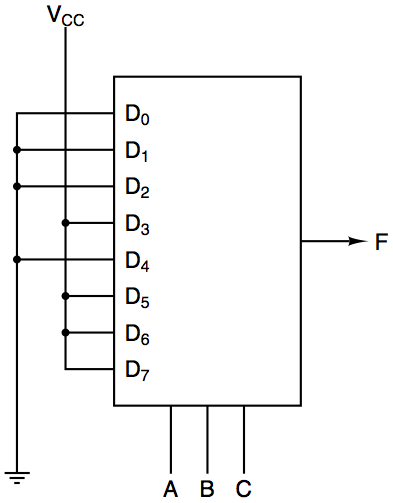
\includegraphics[width=6cm]{tobbsegifvmux}
	\caption{Többségi függvény megvalósítása multiplexerrel.\label{fig:tobbsegifvmux}}
\end{figure}

\paragraph{Demultiplexer} A multiplexer fordítottja. $1$ adatbemenete, $2^n$ adatkimenete és $n$ vezérlőbemenete van, utóbbi határozza meg, hogy az adatbemenet jele melyik adatkimeneten jelenik meg.

\subsubsection{Dekódolók}

Bemenetük egy $n$-bites szám, kimenetük $2^n$ darab jel, ezek közül a bemenetek egyet kiválasztanak, és azt $1$-re állítják. A példán (\ref{fig:dekodolo}. ábra) az $n=3$ eset szerepel. Dekódolót használhatunk pl. akkor, ha 8 db. 1 MB-os memórialapkánk van, és ezek bájtjait egységesen szeretnénk címezni. Ekkor a memóriacím felső 3 bitje egy dekódoló vezérlőjele lehet, amely a lapkát választja ki.

\begin{figure}[htbp]
	\centering
		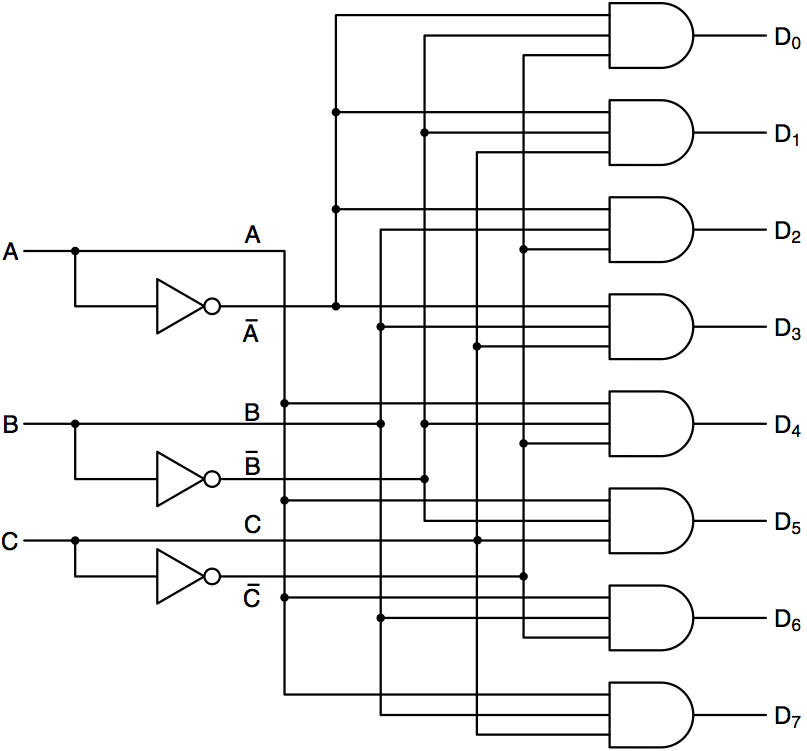
\includegraphics[width=10cm]{dekodolo}
	\caption{3-8 dekódoló.\label{fig:dekodolo}}
\end{figure}

\subsubsection{Összehasonlítók}

Két bemenet bitenkénti összehasonlítását végzik. Egy kétbites összehasonlító logikai kapcsolása az~\ref{fig:osszehasonlito}. ábrán látható.

\begin{figure}[htbp]
	\centering
		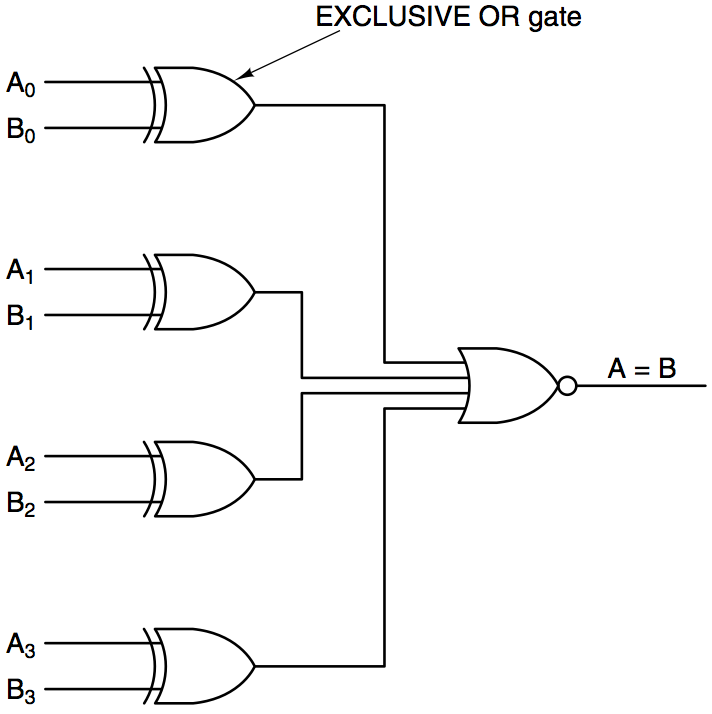
\includegraphics[width=8cm]{osszehasonlito}
	\caption{2-bites összehasonlító.\label{fig:osszehasonlito}}
\end{figure}

\subsection{Programozható logikai tömb (PLA). Aritmetikai áramkörök. Összeadók. Aritmetikai-logikai egység. Órák.}

\subsubsection{Programozható logikai tömb (PLA)}

Nagyon általános lap. Példánkon (\ref{fig:pla}. ábra) egy 12-bemenetes PLA látható, ennek valójában 24 bemenete van, mert a lapka mindegyiket negálja is. A bemenetek 50, egyenként 24-bemenetű \textsc{and}-kapuba vannak kötve egy-egy olvadóbiztosítékon keresztül. Az \textsc{and}-kapuk kimenetei ezután -- szintén biztosítékokon át -- \textsc{or}-kapukba futnak be. Programozáskor a kiválasztott bitosítékok kiégethetők, így nagyon sokféle logikai függvény megvalósítható.

\begin{figure}[htbp]
	\centering
		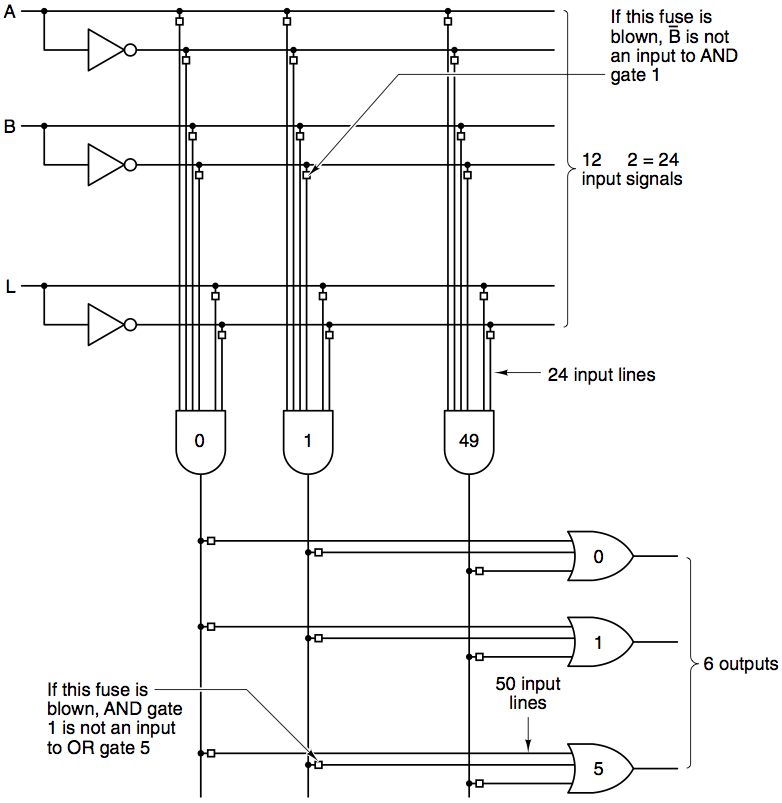
\includegraphics[width=8cm]{pla}
	\caption{12-bemenetes, 6-kimenetes programozható logikai tömb.\label{fig:pla}}
\end{figure}

\subsubsection{Aritmetikai áramkörök. Összeadók.}

\paragraph{Léptető} Egy 8-bites szám bináris számjegyeit tolja bitenként jobbra vagy balra. 8 bemenete ($D_0, D_1, \dots$), 8 kimenete ($S_1, S_2, \dots$) és egy vezérlőjele ($C$) van. Utóbbi 1 értéke esetén jobbra, 0 értékénél balra tolódnak a számjegyek. Ld.~\ref{fig:lepteto}. ábra.

\begin{figure}[htbp]
	\centering
		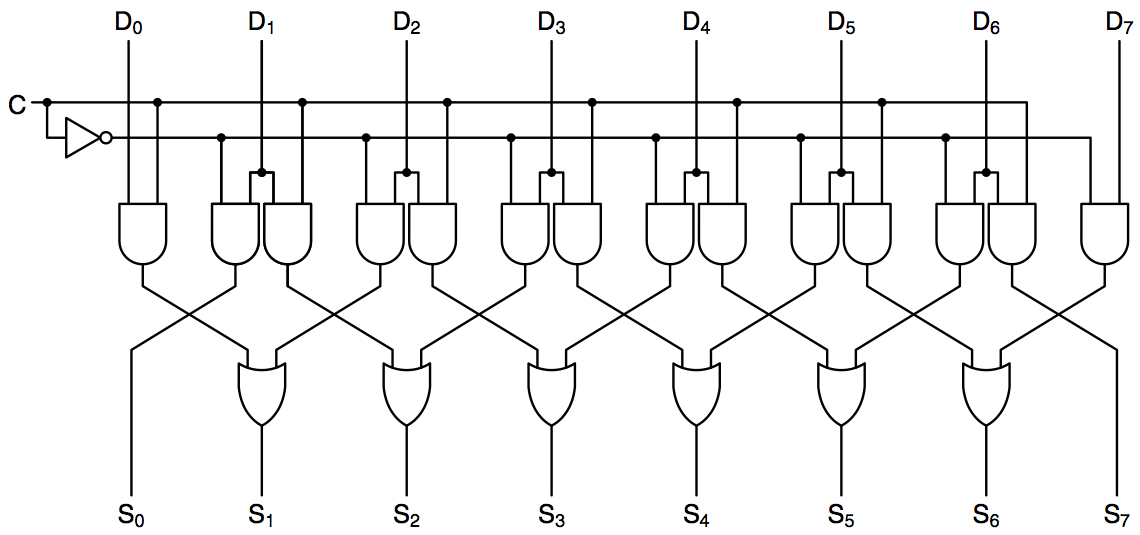
\includegraphics[width=8cm]{lepteto}
	\caption{8-bites léptető.\label{fig:lepteto}}
\end{figure}

\paragraph{Félösszeadó} Két egybites számot tud összeadni, kimenete az eredmény és az átvitel. Átvitelbemenete nincs, ezért nem lehet összekapcsolni más félösszeadókkal. Ld.~\ref{fig:felosszeado}. ábra.

\begin{figure}[htbp]
	\centering
		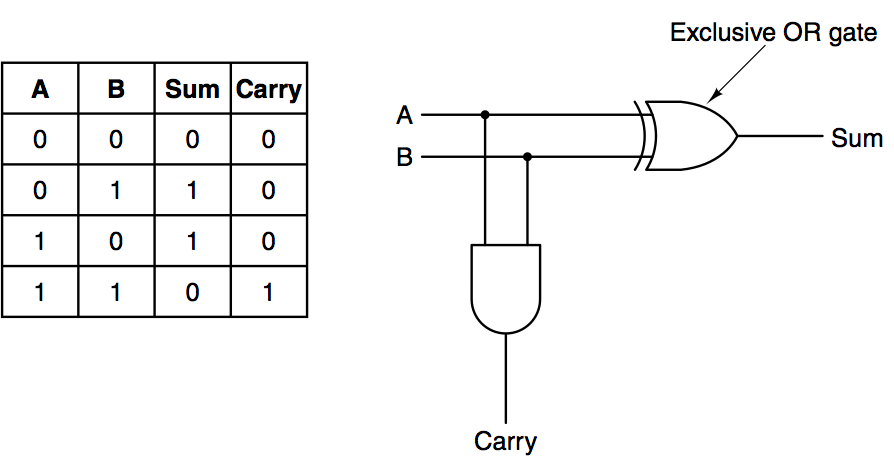
\includegraphics[width=8cm]{felosszeado}
	\caption{Egybites egészek összeadásának igazságtáblája. Félösszeadó.\label{fig:felosszeado}}
\end{figure}

\paragraph{Teljes összeadó} Két félösszeadóból épül fel. Az összeg akkor $1$, ha az A, B és átvitel bemeneteken páratlan az $1$-esek száma. Az átvitelkimenet $1$, ha A és B is $1$, vagy pontosan egyikük $1$, és az átvitelbemenet is $1$.

\begin{figure}[htbp]
	\centering
		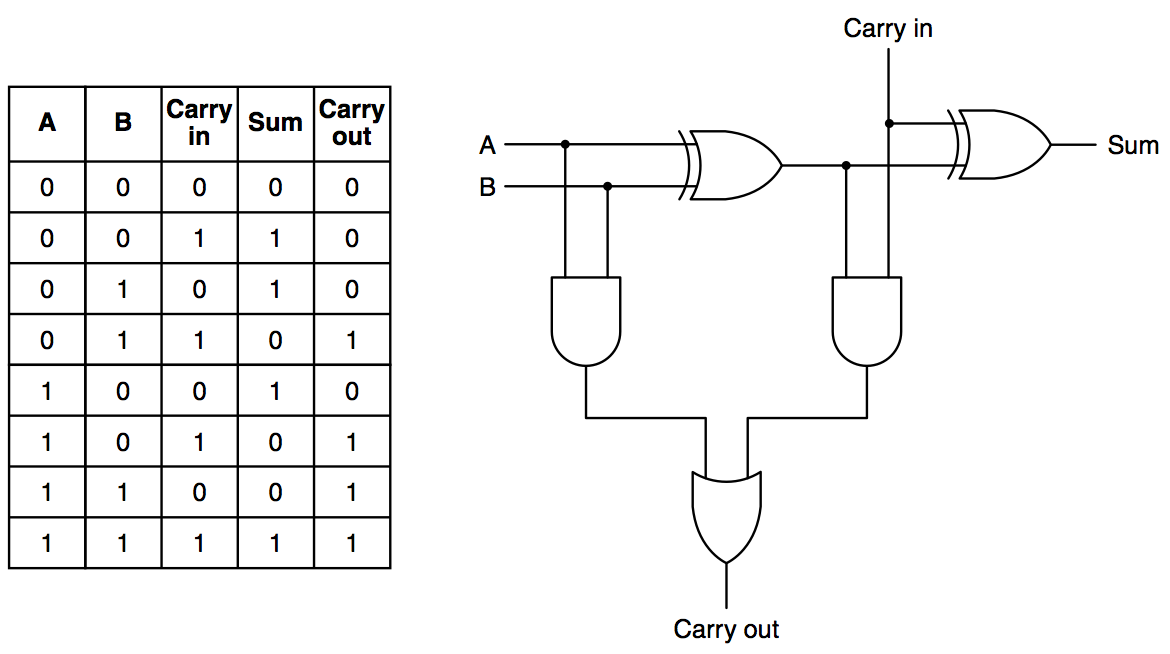
\includegraphics[width=10cm]{teljesosszeado}
	\caption{Teljes összeadó igazságtáblája és kapcsolása.\label{fig:teljesosszeado}}
\end{figure}

\paragraph{Összetett összeadó} 16-bites szó összeadásához elég 16 teljes összeadót összekapcsolnunk: az átvitelkimeneteket a bal oldali szomszéd átvitelbemenetére kötjük. Így az átvitel végighalad az elemi összeadókon, legrosszabb eset az $111\dots111+1$ összeg kiszámítása. Az eredményt csak bizonyos késleltetés után kapjuk meg. Vannak olyan összeadók, amelyeknél nincs ilyen késleltetés.

32-bites összeadó működését úgy gyorsíthatjuk, hogy 3 16-bitessel helyettesítjük. Az alsó helyiértékeket $A_1$ adja össze, a felsőket pedig vele párhuzamosan $A_2$ és $A_3$, egyikük úgy, mintha lett volna átvitel, másikuk úgy, mintha nem. $A_2$ és $A_3$ értéke közül $A_1$ átvitelkimenete választja ki az érvényeset. Az ilyet \emph{átvitelkiválasztó összeadónak} nevezzük.

\subsubsection{Aritmetikai-logikai egység}

Olyan áramkör, amely \textsc{és} és \textsc{vagy} műveleteket hajt végre, és két gépi szót összead. $n$-bites szavak esetén $n$ azonos áramkört tartalmaz.

\paragraph{1-bites ALU} Kétbites dekódere $F_0$ és $F_1$ vezérlőjeleivel kiválaszthatjuk a kívánt műveletet: $A \land B$, $A \lor B$, $\lnot B$, vagy $A+B$. Az A és B bemenő jeleket az ENA és ENB vezérlőjelekkel engedélyezhetjük. Bemenet még A negáltja és az átvitel, kimenet a művelet eredménye és az átvitel. Ld.~\ref{fig:1bitalu}. ábra.

\begin{figure}[htbp]
	\centering
		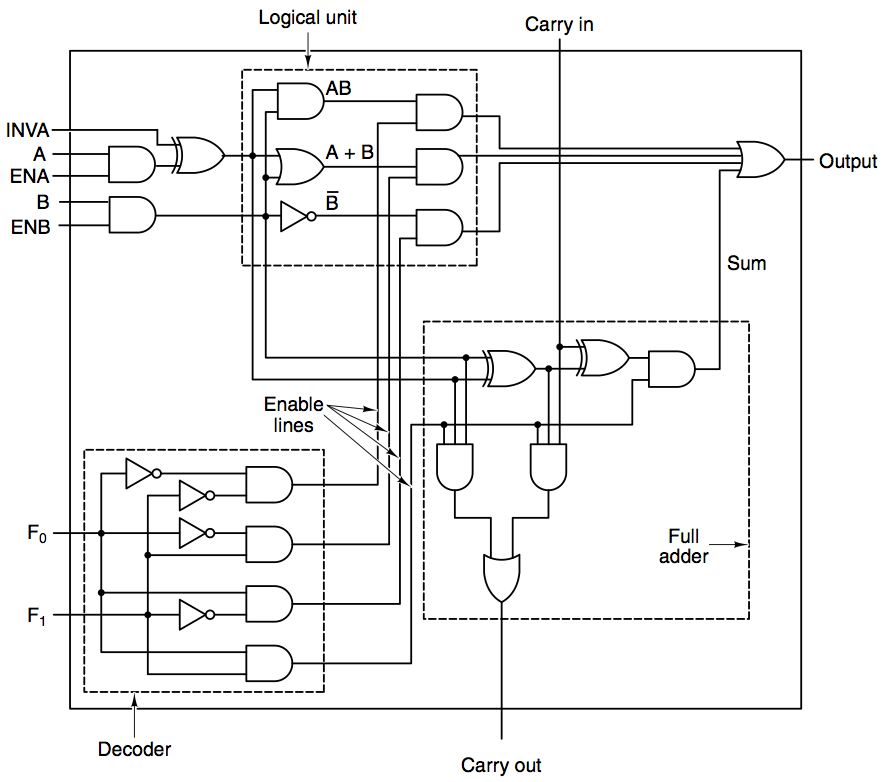
\includegraphics[width=10cm]{1bitalu}
	\caption{1-bites aritmetikai-logikai egység.\label{fig:1bitalu}}
\end{figure}

\paragraph{8-bites ALU} Bitszelet-áramkörökből (1-bites ALU-kból) lehet felépíteni (az invertáló jelek nincsenek feltüntetve). INC bemenete az eredményt eggyel növeli. Ld.~\ref{fig:1bitalu}. ábra.

\begin{figure}[htbp]
	\centering
		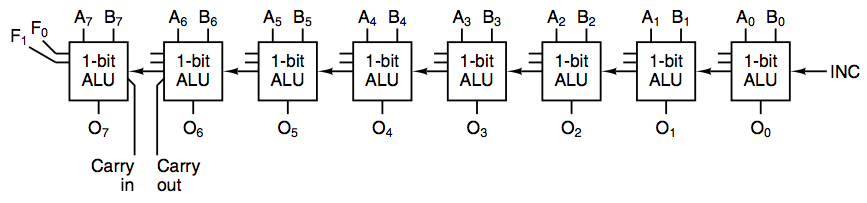
\includegraphics[width=10cm]{8bitalu}
	\caption{8-bites aritmetikai-logikai egység.\label{fig:8bitalu}}
\end{figure}

Sok digitális áramkörben kritikus az események sorrendje. Egyes eseményeknek egymás után, másoknak párhuzamosan kell bekövetkeznie. Sok digitális áramkör órát használ a szinkronizációra. Itt az \emph{óra} olyan áramkört jelent, amely impulzusok sorozatát bocsátja ki állandó, pontos impulzusszélességgel és -közzel. Két szomszédos impulzus közötti idő a \emph{ciklusidő}. Ld.~\ref{fig:ora}. ábra.

\begin{figure}[htbp]
	\centering
		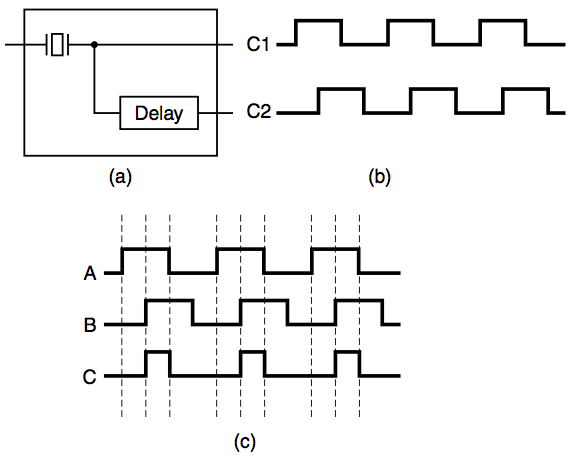
\includegraphics[width=8cm]{ora}
	\caption{(a) Óra (b) idődiagramja. (c) Aszimmetrikus órajelgenerálás.\label{fig:ora}}
\end{figure}

Finomabb felbontás elérése érdekében az órajelet gyakran ``megcsapolják'', és késleltető áramkörrel eltolják, így \emph{másodlagos órajelet} létrehozva. Így egy ciklus alatt négy időbeli referenciapontot kapunk: $C_1$ és $C_2$ fel- és lefutó éleit. Egyes áramkörökben elég, ha az események csak adott időintervallumon belül történnek meg, pl. amikor $C_1$ magas, nem kell pontosan a felfutó élhez időzíteni. Az órák általában \emph{szimmetrikusak}: ugyanannyi időt töltenek magas és alacsony állapotban egy cikluson belül. Aszimmetrikus órajel előállításához egy szimmetrikus jel és fáziseltolt változata \textsc{és}-kapcsolatát képezzük.

\end{document}